\documentclass[11pt,a4paper]{article}
\usepackage[a4paper,margin=1.9cm]{geometry}
\usepackage{graphicx}
\usepackage{amsmath}
\usepackage{amssymb}
\usepackage{bm}
\usepackage[numbers,sort&compress]{natbib}
\usepackage{hyperref}
\usepackage{xcolor}
\usepackage{setspace}
\usepackage{placeins}   % \FloatBarrier at the end of sections

% Compatibility shims for revtex commands used in the body
\newcommand{\affiliation}[1]{\\[2pt]\small\itshape #1\normalfont}
\newenvironment{acknowledgments}{\par\noindent\textbf{Acknowledgments.}\ }{\par}
\newenvironment{widetext}{}{}

% Allow figures to fill a higher fraction of the page (default is 70%)
% so they stop accumulating at the end of the document.
\renewcommand{\topfraction}{0.9}
\renewcommand{\bottomfraction}{0.8}
\renewcommand{\textfraction}{0.1}
\renewcommand{\floatpagefraction}{0.8}
% \subequations works via amsmath, already loaded

\hypersetup{
  colorlinks=true,
  linkcolor=blue,
  citecolor=blue,
  urlcolor=blue
}

% ---- Typography: open up vertical rhythm for readability ----
\linespread{1.08}           % Modest line-spacing increase (~8%)
\setlength{\parskip}{2pt plus 1pt minus 0.5pt}

% Extra breathing room around display math
\setlength{\abovedisplayskip}{10pt plus 2pt minus 2pt}
\setlength{\belowdisplayskip}{10pt plus 2pt minus 2pt}
\setlength{\abovedisplayshortskip}{8pt plus 2pt minus 2pt}
\setlength{\belowdisplayshortskip}{8pt plus 2pt minus 2pt}

% More space around figures
\setlength{\textfloatsep}{14pt plus 2pt minus 2pt}
\setlength{\floatsep}{14pt plus 2pt minus 2pt}
\setlength{\abovecaptionskip}{8pt}
\setlength{\belowcaptionskip}{4pt}

% Slightly enlarged section spacing
\makeatletter
\renewcommand\section{\@startsection{section}{1}{\z@}%
  {-2.5ex \@plus -1ex \@minus -.2ex}%
  {1.8ex \@plus.2ex}%
  {\normalfont\normalsize\bfseries\centering}}

% More vertical room around \paragraph* headings so "Crossover..." etc.
% don't visually merge with the paragraph before them
\renewcommand\paragraph{\@startsection{paragraph}{4}{\z@}%
  {1.2ex \@plus 0.3ex \@minus .2ex}%
  {-0.6em}%
  {\normalfont\normalsize\itshape}}
\makeatother

\begin{document}

\title{Angular persistence and the universal pre-asymptotic
       Hurst exponent of thermal soaring flights}

\author{Matteo Di Sante\\[2pt]
\small\itshape Dipartimento di Fisica ``Enrico Fermi'',
Universit\`a di Pisa, Largo Bruno Pontecorvo 3, 56127 Pisa, Italy\normalfont}

\date{April 24, 2026}

\renewenvironment{abstract}{\small\begin{quote}\textbf{Abstract.} }{\end{quote}\normalsize}

\maketitle

\begin{abstract}
A recent empirical analysis [J.\ Vilpellet, A.\ Darmon and
M.\ Benzaquen, arXiv:2601.01293 (2026)] reports a sub-ballistic
Hurst exponent $H \approx 0.88$ for horizontal transport in
paraglider, hang glider and sailplane flights that is essentially
independent of aircraft type, despite sizeable differences in
characteristic horizontal speed and in the Pareto-tail exponents
of the transition- and search-phase duration distributions. We
introduce a minimal cycle-based continuous-time random walk
(CTRW) model in which each elementary step is a complete
transition--search--climb cycle. Phase durations are i.i.d.\ with
Pareto tails for transition and search (tail exponents
$\mu_{\mathrm{T}},\mu_{\mathrm{S}}>1$ taken from the reference
analysis) and an exponential law for climb. Each phase carries
its own intra-phase horizontal dynamics, independently specified:
a ballistic translation during transition; an intermittent
two-state motion during search, in which exponential-duration
ballistic repositioning legs alternate with
Mittag--Leffler-distributed localised scouting rests; and a 2-D
harmonic oscillator with per-cycle turn-period dispersion plus a
weak orographic drift during climb. Successive transition
headings evolve by a Gaussian random walk on the circle with
per-cycle variance $\sigma_\theta^2$. A closed-form expression
for the discrete-step mean-square displacement (MSD) is derived,
exhibiting a pre-asymptotic crossover window in which a single
power-law fit yields effective Hurst exponents in $(1/2,1)$. The
$(\mu_{\mathrm{T}},\sigma_\theta)$ phase diagram of the model
places the iso-line $H_{\mathrm{eff}}=0.88$ at $\sigma_\theta
\simeq 0.35\,\mathrm{rad}$ essentially independently of
$\mu_{\mathrm{T}}$, supplying an analytical origin for the
observed universality. Monte Carlo simulations at this
universal $\sigma_\theta$ reproduce the empirical MSD with a
tight aircraft-to-aircraft spread $\Delta H \lesssim 0.01$:
paragliders $H=0.934$, hang gliders $H=0.930$, sailplanes
$H=0.937$. Rescaling by $v_{xy}^2$ collapses the three curves
onto a single master function of the lag, reproducing the
universal collapse reported experimentally (inset of
Fig.~1 of the reference analysis). The paraglider intra-phase
parameters are calibrated on Fig.~3 of the reference analysis;
hang-glider and sailplane Pareto scales $\tau_0^{\mathrm{T}},
\tau_0^{\mathrm{S}}$ (which the reference analysis does not
publish) are tuned so that $\langle\tau^{\mathrm{T}}\rangle$
and $\langle\tau^{\mathrm{S}}\rangle$ match the paraglider
values, thereby collapsing $\delta^2(\Delta)/v_{xy}^2$;
$\sigma_\theta$ is imposed analytically from the phase diagram
rather than fitted.
\end{abstract}

\section{Introduction}

Anomalous transport in heterogeneous, patchy, and intermittent
environments is a recurrent theme in physics, biology and
ecology~\cite{metzler2000,zaburdaev2015,codling2008,benichou2011}.
Cross-country soaring flight provides a natural instance: paragliders,
hang gliders and sailplanes exploit atmospheric thermal updrafts as
localised energy patches, alternating ballistic glides between
thermals with localised circling motion inside them. Large GPS
trajectory archives have recently enabled population-scale
statistical analyses of the resulting transport~\cite{vilpellet2026}.

In a comprehensive empirical study, Vilpellet, Darmon and
Benzaquen~\cite{vilpellet2026} analysed $49\,939$ paraglider, $780$
hang-glider and $9\,203$ sailplane trajectories and reported a
striking observation: beyond a short ballistic regime
($\Delta \lesssim 10$\,s), the horizontal MSD grows as
$\delta^2(\Delta) \propto \Delta^{2H}$ with $H \approx 0.88$ for
\emph{all three} aircraft types. This is non-trivial in view of the
differences in horizontal velocity $v_{xy}$ (factor $\sim 3.6$
between paragliders and sailplanes) and in the empirical tail
exponents of the phase-duration distributions (factor $\sim 1.8$ in
$\mu_T$, see Table~\ref{tab:params}).

Using a hidden Markov model~\cite{rabiner1989}, the authors
of~\cite{vilpellet2026} segmented each flight into repeating
transition--search--climb cycles and showed that within each phase
the motion has well-defined but very different scaling: transition
phases are individually ballistic, search phases are strongly
subdiffusive, and climb phases produce very little net horizontal
displacement --- approximately two orders of magnitude below $v_{xy}$
according to~\cite{vilpellet2026} --- because thermal updrafts are
typically tilted by ambient wind and breeze, causing a slow drift
rather than true vertical motion.

In their Discussion, Vilpellet \emph{et al.}~\cite{vilpellet2026}
discuss a L\'evy-walk-type mechanism~\cite{zaburdaev2015} as a
candidate explanation, noting that in this regime one would expect
$\delta^2 \sim \Delta^{4-\mu}$ (density-convention formula) and that
the observed $H = 0.88$ would correspond to $\mu \approx 2.25$. They
note however that the measured $\mu_T$ values differ across aircraft
while the Hurst exponent does not, incompatible with a naive
aircraft-by-aircraft L\'evy-walk interpretation. They conclude that
``two-dimensional directional decorrelation'' and
``pre-asymptotic scaling''~\cite{metzler2000,meroz2015} must also
play a role but leave the quantitative modelling as an open problem.
In addition, the Fig.~4 caption of~\cite{vilpellet2026} declares the
survival convention $P(\tau>t)\sim t^{-\mu}$, whereas the
$\Delta^{4-\mu}$ formula and the statement ``$\mu<3$, infinite
variance'' in their text tacitly assume the density convention
$f(\tau)\sim\tau^{-\mu}$, an internal ambiguity we address
explicitly (Appendix~A).

In this Letter we show that a minimal cycle-based CTRW model with an
explicit angular-persistence mechanism reproduces the observed
universality quantitatively. We derive a closed-form expression for
the MSD after $N$ cycles (App.~C); characterise a pre-asymptotic
crossover window --- the range of time lags in which the system has
not yet reached its diffusive asymptotics --- over which a single
power-law fit yields an effective exponent $H_{\mathrm{eff}} \in
(1/2, 1)$; and map out the $(\mu_T,\sigma_\theta)$ phase diagram of
$H_{\mathrm{eff}}$. The phase diagram exhibits nearly horizontal
isocurves of $H_{\mathrm{eff}}$ (Fig.~\ref{fig:phase}) and locates
the empirical $H=0.88$ contour at $\sigma_\theta\simeq
0.35\,\mathrm{rad}$, essentially independent of $\mu_T$; we identify
this weak $\mu_T$-dependence as the analytical origin of the
universality. A direct Monte Carlo simulation of the full model with
this angular diffusivity, using paragliders intra-phase
parameters tuned on Fig.~3 of~\cite{vilpellet2026} and the
parameters of Table~\ref{tab:params} for the other two aircraft
classes, yields $H=0.934,\,0.930,\,0.937$ respectively
(fitted in $10\,\mathrm{s}<\Delta<5\times10^3\,\mathrm{s}$).
Rescaling by $v_{xy}^2$ collapses the three MSD curves onto a
single master function of the lag (Fig.~\ref{fig:msd-rescaled}),
reproducing the universal transport reported experimentally in
the inset of Fig.~1 of~\cite{vilpellet2026}.

\begin{table}[!htbp]
\centering
\small
\begin{tabular}{lccc}
\hline\hline
 & paragliders & hang gliders & sailplanes \\
\hline
$v_{xy}$ (m/s)                  & $10.06$ & $15.58$ & $35.85$ \\
$\mu_{\mathrm{T}}$ (transition) & $3.93$  & $4.79$  & $2.62$ \\
$\mu_{\mathrm{S}}$ (search)     & $3.88$  & $2.25$  & $2.90$ \\
$\mu_{\mathrm{C}}$ (climb)      & $8.28$  & $5.33$  & $4.54$ \\
$\eta_{\mathrm{T}}$ (trans.\ fraction) & $0.61$ & $0.56$ & $0.58$ \\
$\eta_{\mathrm{S}}$ (search fr.)       & $0.06$ & $0.05$ & $0.015$ \\
$\eta_{\mathrm{C}}$ (climb fr.)        & $0.32$ & $0.39$ & $0.40$ \\
$H_{\mathrm{obs}}$ & \multicolumn{3}{c}{$0.88$ (universal)} \\
\hline\hline
\end{tabular}
\caption{Empirical parameters from~\cite{vilpellet2026}. Tail
exponents $\mu$ of phase durations are Hill-estimator values
reported in the legend of Fig.~4c,f,i of the cited paper; under
our convention (Appendix~A) $\langle \tau
\rangle<\infty$ requires $\mu>1$ and $\langle \tau^2\rangle<\infty$
requires $\mu>2$, so all aircraft have finite variance of phase
durations. Time fractions $\eta$ are ensemble means read from the
pie charts in Fig.~7 of~\cite{vilpellet2026}. The Pareto scales
$\tau_0^{\mathrm{T}}, \tau_0^{\mathrm{S}}$ of the phase-duration
distributions are model-introduced and not published
in~\cite{vilpellet2026}: for paragliders we take physically
plausible values (see configs), for hang gliders and sailplanes
we tune them so that $\langle\tau^{\mathrm{T}}\rangle$ and
$\langle\tau^{\mathrm{S}}\rangle$ match the paraglider values,
aligning the mean cycle duration $\langle T\rangle$ across
aircraft and collapsing $\delta^2(\Delta)/v_{xy}^2$ onto the
paraglider curve (Fig.~\ref{fig:msd-rescaled}). This alignment
induces minor deviations ($\lesssim 0.1$) from the $\eta_X$
values quoted here.}
\label{tab:params}
\end{table}

\section{The cycle-based CTRW model}
\label{sec:model}

We regard each soaring cycle $n \in \mathbb{N}$ as a single discrete
step of a two-dimensional CTRW~\cite{metzler2000,scalas2004}. The
empirical segmentation of~\cite{vilpellet2026} resolves each flight as
a repeating ordered sequence
\emph{climb}~$\to$~\emph{transition}~$\to$~\emph{search};
after the first search only, every subsequent search is always
preceded by a completed climb. Only the \emph{transition} phase
contributes a net horizontal step in our cycle-based decomposition,
the other two phases being modelled as locally reshuffled motions
that carry no net persistent direction (assumption (A4) below). The
horizontal position at the end of cycle $n$ is therefore
\begin{equation}
\mathbf{x}_n = \mathbf{x}_{n-1} + \ell_n\,\hat{\mathbf{e}}(\theta_n),
\qquad \hat{\mathbf{e}}(\theta) \equiv (\cos\theta,\sin\theta),
\label{eq:step}
\end{equation}
with step length $\ell_n = v_{xy}\,\tau_n^{\mathrm{T}}$ set by the
transition duration. The cycle duration is $T_n = \tau_n^{\mathrm{T}}
+ \tau_n^{\mathrm{S}} + \tau_n^{\mathrm{C}}$, and the cycle-count
process is $N(t) = \max\{n : \sum_{k \le n} T_k \le t\}$.

The model is fully specified by the following assumptions, each an
explicit modelling choice on top of the CTRW framework itself:

\begin{description}
\setlength{\itemsep}{1.2ex}
\item[\textbf{(A1)}] \emph{Cycle statistics.} The triples
$\{(\tau_n^{\mathrm{T}}, \tau_n^{\mathrm{S}}, \tau_n^{\mathrm{C}})\}_n$
are i.i.d.\ with independent marginals. The empirical survival
functions of Fig.~4c,f,i of~\cite{vilpellet2026} display heavy
power-law tails for transition and search and a light exponential
tail for climb; accordingly we parametrise
\begin{equation}
P(\tau^{X}>\tau)=\bigl(\tau_{\min}^{X}/\tau\bigr)^{\mu_X},\quad
\tau\ge\tau_{\min}^{X},\ X\in\{\mathrm{T},\mathrm{S}\},
\label{eq:pareto}
\end{equation}
(a Pareto tail in the survival convention of Fig.~4
of~\cite{vilpellet2026}), and
$\tau^{\mathrm{C}} \sim \mathrm{Exp}(\bar{\tau}_{\mathrm{C}})$,
with tail exponents $\mu_X$ taken directly from the Hill fits of
Fig.~4c,f,i of~\cite{vilpellet2026} (Table~\ref{tab:params}).
The scale parameters $\tau_{\min}^{X}$ are modelling choices (not
read from~\cite{vilpellet2026}) set so that the resulting mean
durations sit in a realistic range; see the code configuration
files. All empirical $\mu_X$ are $>1$ (Table~\ref{tab:params}), so
$\langle\tau^{X}\rangle$ is finite; the more general
Mittag--Leffler CTRW framework~\cite{metzler2000,scalas2004}, valid
for $\mu_X\in(0,1)$, thus reduces here to its Pareto tail, and we
work with Eq.~\eqref{eq:pareto} directly. The Mittag--Leffler law
itself plays a different role in the model, deferred to the
search-phase dynamics (A2.S) below.

\item[\textbf{(A2)}] \emph{Intra-phase horizontal motion.} During the
transition phase of cycle $n$ the aircraft moves deterministically
at velocity $v_{xy}\,\hat{\mathbf{e}}(\theta_n)$, producing a
ballistic MSD $\delta^2_T(\Delta) = v_{xy}^2 \Delta^2$ at all lags
below $\tau^T_n$. The search and climb phases are modelled
differently because their empirical MSDs in Fig.~3
of~\cite{vilpellet2026} display qualitatively different features:
\begin{description}
\item[(A2.S) Search: intermittent ballistic CTRW with
Mittag-Leffler rests.] Inside each search phase of duration
$\tau^S_n$, the pilot's horizontal motion in the
$xy$-plane alternates between two physically distinct regimes:
\begin{enumerate}
\setlength{\itemsep}{0.5ex}
\item \emph{Ballistic legs} of duration
$\sigma_k \sim \mathrm{Exp}(\sigma_0)$, during which the walker
translates at effective speed $v_c^S > v_{xy}$ in the $xy$-plane
along a persistent direction $\psi_k$ (intra-phase angular
Gaussian random walk on the circle,
$\psi_k = \psi_{k-1} + \zeta_k$, $\zeta_k \sim \mathcal{N}(0,
\sigma_\psi^2)$; not to be confused with the cycle-to-cycle angular
increment $\eta_n\sim\mathcal{N}(0,\sigma_\theta^2)$ of (A3) below).
\item \emph{Waiting epochs} of duration
$\xi_k$ drawn from a Mittag-Leffler distribution,
\begin{equation}
P(\xi_k > \xi)
= E_{\alpha_S}\!\left[-(\xi/\tau_0^S)^{\alpha_S}\right],
\label{eq:ml-wait}
\end{equation}
with $\alpha_S \in (0, 1)$, during which the walker's horizontal
position does not advance on the scale of the GPS sampling.
\end{enumerate}
This two-component dynamics is a \emph{CTRW with finite-velocity
(ballistic) steps of duration $\sigma_k$ and Mittag--Leffler
waiting times $\xi_k$}~\cite{scalas2004,metzler2000}. Because
$\sigma_k$ is exponentially distributed the individual steps are
not heavy-tailed, and this process is therefore \emph{not} a
Lévy walk~\cite{zaburdaev2015} (whose legs would be power-law in
duration): the sub-diffusive long-time behaviour arises entirely
from the heavy-tailed waits $\xi_k$. The CTRW admits a rigorous
continuum-limit representation as a subordinated process,
\begin{equation}
\mathbf{X}^S(t) \;=\; \tilde{\mathbf{X}}^S\bigl(E_{\alpha_S}(t)\bigr)
\quad\text{(in distribution, at $t\gg\tau_0^S$)},
\label{eq:subord}
\end{equation}
where $\tilde{\mathbf{X}}^S(\cdot)$ is the leg-count-indexed
displacement process and $E_{\alpha_S}(t)$ is the inverse of a
one-sided $\alpha_S$-stable subordinator, the continuum limit of
the Mittag--Leffler renewal counting process. A self-contained
derivation --- Laplace-transform analysis of the renewal density
and the Meerschaert--Scheffler~\cite{meerschaert2004} limit
theorem --- is given in Appendix~H.

\textbf{Physical interpretation of the waiting times
(modelling hypothesis).}
The following is a \emph{modelling interpretation}, not a feature
extracted from the data of~\cite{vilpellet2026}: the raw
trajectories were segmented into three phases via a hidden Markov
model~\cite{rabiner1989} and no further sub-segmentation of the
search phase is reported there. We propose the following reading
of the two-component CTRW of (A2.S). The pilot is \emph{never
strictly at rest} --- a paraglider, hang glider or sailplane
cannot hover. We therefore hypothesise that the waiting epochs
$\xi_k$ of (A2.S) correspond to the horizontal projection of a
\emph{localised circling motion} that the pilot performs while
probing a candidate updraft. Under this hypothesis, during each
``tight-scouting'' epoch the pilot circles in place at an
effective radius $r^{\mathrm{scout}} \ll r_0^{\mathrm{climb}}$
(assumed of order a few metres) with a short turn period (assumed
of order a few seconds), much faster than the thermalling turn of
the climb phase. In the $xy$-projection at GPS sampling rate
($\Delta t \sim 1$\,s), such tight circling would produce a
position signal fluctuating at an amplitude below the effective
spatial resolution of the sampled trajectory, and would therefore
be observationally indistinguishable from a pause --- consistent
with the HMM output but not directly confirmed by it.
The broad Mittag-Leffler distribution of the $\xi_k$ is then a
further hypothesis, reflecting a broad range of scouting times
invested on different candidate spots (from quick discard,
$\xi \sim 1$\,s, to prolonged evaluation, $\xi \sim$ minutes);
the empirical intra-search MSD of Fig.~3e
of~\cite{vilpellet2026} is consistent with this heavy-tailed
waiting-time ansatz but does not by itself pin down the full
distribution.

The ballistic legs, in turn, are interpreted --- again as a
modelling hypothesis --- as short tactical manoeuvres, i.e.\
repositioning glides between neighbouring scouting spots. Their
effective speed $v_c^S > v_{xy}$ is taken so that during a pure
repositioning glide the pilot, not circling, moves faster in the
$xy$-plane than the cycle-averaged horizontal speed $v_{xy}$
(which incorporates the tight-circling periods). The exponential
law for $\sigma_k$ is chosen for minimality (memoryless
manoeuvres); it is not a direct empirical observation of
individual leg durations, which are not resolved separately in
the HMM output.

With Mittag-Leffler waits and exponential legs, the MSD of (A2.S)
has three regimes separated by the two timescales $\sigma_0$ and
$\tau_0^S$:
\begin{equation}
\delta^2_S(\Delta) \sim
\begin{cases}
 (v_c^S)^2\,\Delta^2 & \Delta \ll \sigma_0 \\
 \text{transient} & \sigma_0 \ll \Delta \ll \tau_0^S \\
 \frac{(v_c^S\sigma_0)^2}{\Gamma(1+\alpha_S)}
  \left(\frac{\Delta}{\tau_0^S}\right)^{\alpha_S}
 & \Delta \gg \tau_0^S,
\end{cases}
\label{eq:msd-search-subdiff}
\end{equation}
where the first regime is the ballistic short-time inertial motion
inside a single leg and the third is the asymptotic sub-diffusive
scaling of the Mittag-Leffler CTRW, recovering the empirical exponent
$\alpha_S = 0.6$ (paragliders, hang gliders) or $\alpha_S = 0.4$
(sailplanes) reported in Fig.~3 of~\cite{vilpellet2026}. The
transient regime has an effective exponent between 1 and
$\alpha_S$, depending on $\sigma_0/\tau_0^S$. A derivation of the
three regimes by direct ensemble averaging of the leg-count
renewal process is given in App.~G.
\item[(A2.C) Climb: 2D harmonic oscillator plus drift with
per-cycle turn-period dispersion.] Inside each climb phase of
duration $\tau^C_n$, the pilot circles a thermal core at a fixed
aircraft-specific radius $r_0$ with an angular frequency
$\omega_{0,n} = 2\pi/T_{\mathrm{turn},n}$ that fluctuates
cycle-to-cycle,
\begin{equation}
T_{\mathrm{turn},n} \sim \mathcal{N}(\bar{T},\sigma_T^2),
\quad\text{clipped at}\ T_{\mathrm{turn},n}\ge 0.2\,\bar{T},
\label{eq:Tturn-Gaussian}
\end{equation}
with $(\bar{T},\sigma_T)=(60,35)$\,s for paragliders and hang
gliders and $(\bar{T},\sigma_T)=(30,5)$\,s for sailplanes in the
configurations used in Figs.~\ref{fig:msd}--\ref{fig:msd-phase}. The circling is
superposed on a linear orographic drift of magnitude
$v_{\mathrm{drift}} \ll v_{xy}$:
\begin{equation}
\mathbf{x}^C_n(c) = r_0\,\bigl[
  \hat{\mathbf{R}}(\omega_{0,n} c + \phi_{0,n}) - \hat{\mathbf{R}}(\phi_{0,n})
\bigr] + v_{\mathrm{drift}}\,c\,\hat{\mathbf{e}}(\phi_n^{\mathrm{drift}}),
\label{eq:climb-oscillator}
\end{equation}
where $\hat{\mathbf{R}}(\phi) = (\cos\phi, \sin\phi)$, $\phi_{0,n}$
is an initial circling phase uniform on $[0, 2\pi)$, and
$\phi_n^{\mathrm{drift}}$ is a drift direction drawn i.i.d.\
uniformly per cycle. The conditional MSD \emph{at fixed}
$T_{\mathrm{turn},n}$ (derived in Sec.~\ref{sec:msd} below),
\begin{equation}
\delta^2_C(\Delta \mid \omega_{0,n}) = 2 r_0^2 [1 - \cos(\omega_{0,n}\Delta)]
                   + v_{\mathrm{drift}}^2\,\Delta^2,
\label{eq:msd-climb-analytic}
\end{equation}
averaged over the Gaussian dispersion Eq.~\eqref{eq:Tturn-Gaussian},
yields
\begin{equation}
\delta^2_C(\Delta) = 2 r_0^2 \bigl[1 - \langle\cos(\omega_{0}\Delta)\rangle_T\bigr]
                   + v_{\mathrm{drift}}^2\,\Delta^2,
\label{eq:msd-climb-avg}
\end{equation}
so that the per-cycle $\omega_0$ dispersion \emph{damps} the
coherent oscillations of the deterministic-$\omega_0$ version
beyond the first cycle. The MSD exhibits the three regimes of
Fig.~3(a)-(c) of~\cite{vilpellet2026}: ballistic at
$\Delta \ll 1/\bar{\omega}_0$ (tangent speed
$v_t = r_0 \bar{\omega}_0$), a single residual anti-correlation
dip at $\Delta \sim \pi/\bar{\omega}_0$ (visible for the largest
$r_0$), and a quasi-ballistic drift-dominated tail at
$\Delta \gg 1/\bar{\omega}_0$.
\end{description}
The thermalling radius $r_0$ is taken from Fig.~4h
of~\cite{vilpellet2026} and is an aircraft-specific
\emph{constant} in our model ($50$, $58.1$, $129.9$\,m for paragliders,
hang gliders, sailplanes); the mean turn period $\bar{T}$ is
$60$\,s for paragliders and hang gliders (chosen so that the
dispersion $\sigma_T = 35$\,s gives
$\sigma_T \bar{\omega}_0 \gtrsim 1$ and the Gaussian damping
smears out the anti-correlation dip, yielding a monotonic
three-regime MSD) and $30$\,s for sailplanes (higher wing-loading,
tighter and steadier circles, residual dip visible in
Fig.~\ref{fig:msd-phase}(c)); the drift magnitude is
aircraft-specific, $v_{\mathrm{drift}} = 1$\,m/s for paragliders
and hang gliders and $v_{\mathrm{drift}} = 0.36$\,m/s for sailplanes,
reflecting the weaker orographic forcing sampled in high-altitude
sailplane flights. Note that the paragliders radius $r_0=50$\,m
differs from the empirical Fig.~4h peak at $\simeq 39$\,m
of~\cite{vilpellet2026} because we take the config value that
best reproduces the anti-correlation dip of the climb-phase MSD in
Fig.~3 of~\cite{vilpellet2026} together with our
$(\bar{T},\sigma_T)$ choice; this is part of the
paraglider-specific tuning summarised in~\S\ref{sec:mc}.

\item[\textbf{(A3)}] \emph{Heading dynamics.} The transition heading
follows a Gaussian random walk on the circle,
\begin{equation}
\theta_n = \theta_{n-1} + \eta_n, \quad
\eta_n \overset{\mathrm{i.i.d.}}{\sim} \mathcal{N}(0, \sigma_\theta^2),
\label{eq:heading}
\end{equation}
with deterministic $\theta_0$. A direct calculation
(Appendix~B) gives
$\langle \cos(\theta_{n+k} - \theta_n)\rangle = \rho^{|k|}$ with
$\rho \equiv \mathrm{e}^{-\sigma_\theta^2/2}$, so the heading
correlator decays exponentially with a persistence length
\begin{equation}
N_p = 2/\sigma_\theta^2
\label{eq:Np}
\end{equation}
in cycle units, i.e.\ $t_p = N_p\langle T\rangle$ in physical time.

\item[\textbf{(A4)}] \emph{Independence of intra-phase directions.}
The leg directions of search and climb, and the drift direction
$\hat{\mathbf{v}}_n^{\mathrm{drift}}$, are mutually independent and
independent of the transition heading $\theta_n$. This hypothesis
separates the \emph{global} directional persistence (carried by the
transition phases) from the \emph{local} isotropic reshuffling that
the pilot performs inside each thermalling and searching bout, and
is the cleanest null assumption consistent with the phase-resolved
statistics of~\cite{vilpellet2026} in the absence of additional
measurements.
\end{description}

\section{Mean-square displacement}
\label{sec:msd}

Under (A1)--(A4) the total horizontal displacement over $N$ cycles
decomposes into three contributions with mutually independent
directions:
\begin{equation}
\mathbf{x}_N
 = \underbrace{\sum_{n=1}^N \ell_n\,\hat{\mathbf{e}}(\theta_n)}_{\mathbf{X}_N^{\mathrm{T}}}
 + \underbrace{\sum_{n=1}^N \Delta\mathbf{X}_n^S}_{\mathbf{X}_N^{\mathrm{S}}}
 + \underbrace{\sum_{n=1}^N \Delta\mathbf{X}_n^C}_{\mathbf{X}_N^{\mathrm{C}}},
\label{eq:xN-decomp}
\end{equation}
where $\Delta\mathbf{X}_n^{S,C}$ are the per-cycle displacements
during the intra-phase dynamics of (A2.S) and (A2.C), each with
i.i.d.\ uniform leg directions. By (A4), cross-terms between
$\mathbf{X}^{T}$, $\mathbf{X}^{S}$ and $\mathbf{X}^{C}$ vanish on
average, and
\begin{equation}
\langle |\mathbf{x}_N|^2 \rangle
 = \langle |\mathbf{X}_N^{\mathrm{T}}|^2 \rangle
 + \langle |\mathbf{X}_N^{\mathrm{S}}|^2 \rangle
 + \langle |\mathbf{X}_N^{\mathrm{C}}|^2 \rangle.
\label{eq:msd-sum}
\end{equation}

\paragraph*{Inter-cycle contribution (transitions).}
Iterating the transition sum, expanding
$|\mathbf{X}_N^{T}|^2 = \sum_{i,j}\ell_i\ell_j
\hat{\mathbf{e}}(\theta_i)\cdot\hat{\mathbf{e}}(\theta_j)$, and
using the independence of $\ell$ and $\theta$ (Appendix~C), one
obtains
\begin{equation}
\langle |\mathbf{X}_N^{\mathrm{T}}|^2 \rangle
 = N\langle \ell^2 \rangle
 + 2\langle \ell \rangle^2
   \sum_{1 \le i < j \le N} \rho^{j-i}.
\label{eq:msd-raw}
\end{equation}
Counting pairs at fixed gap $k = j-i$ gives
$\sum_{1\le i<j\le N}\rho^{j-i} = \sum_{k=1}^{N-1}(N-k)\rho^k$, which
admits the closed form (Appendix~D)
\begin{equation}
\sum_{k=1}^{N-1}(N-k)\rho^k
 = \frac{N\rho}{1-\rho} - \frac{\rho(1-\rho^N)}{(1-\rho)^2}.
\label{eq:geom}
\end{equation}
Combining Eqs.~\eqref{eq:msd-raw}--\eqref{eq:geom} yields the
inter-cycle transition MSD in closed form,
\begin{widetext}
\begin{equation}
\boxed{\;
\langle |\mathbf{X}_N^{\mathrm{T}}|^2 \rangle
 = N\,\langle \ell^2 \rangle
 + \langle \ell \rangle^2
   \left[\, \frac{2N\rho}{1-\rho}
          - \frac{2\rho(1-\rho^N)}{(1-\rho)^2} \,\right].
\;}
\label{eq:msd-T-exact}
\end{equation}
\end{widetext}
Equation~\eqref{eq:msd-T-exact} is exact in $N$, makes no large-$N$
assumption, and is the direct generalisation of the
straight-segment mean-square-displacement formula of correlated
random walks~\cite{kareiva1983}. Two limits follow:

\begin{itemize}
\setlength{\itemsep}{1.4ex}
\item \emph{Ballistic limit, $N \ll N_p$.}
Taylor-expanding
$\rho = 1 - \sigma_\theta^2/2 + \mathcal{O}(\sigma_\theta^4)$
and
$\rho^N = 1 - N\sigma_\theta^2/2 + \mathcal{O}((N\sigma_\theta^2)^2)$,
\begin{equation}
\langle |\mathbf{X}_N^{\mathrm{T}}|^2 \rangle \simeq
\langle \ell \rangle^2\, N^2
\left[\,1 - \tfrac{1}{3}\,N\sigma_\theta^2
         + \mathcal{O}\!\left((N\sigma_\theta^2)^2\right)\,\right],
\label{eq:msd-ballistic}
\end{equation}
so $\langle |\mathbf{X}_N^{\mathrm{T}}|^2\rangle \propto N^2$ to leading
order: the transition walker is quasi-ballistic over fewer than $N_p$
cycles.

\item \emph{Diffusive limit, $N \gg N_p$.} In this regime
$\rho^N \to 0$, and Eq.~\eqref{eq:msd-T-exact} becomes
\begin{equation}
\langle |\mathbf{X}_N^{\mathrm{T}}|^2 \rangle \simeq
 N\!\left[\, \langle \ell^2 \rangle
         + \frac{1+\rho}{1-\rho}\,\langle \ell \rangle^2
         - \langle \ell\rangle^2 \,\right],
\label{eq:msd-diffusive}
\end{equation}
where we rearranged $2\rho/(1-\rho) = (1+\rho)/(1-\rho) - 1$. In
the strongly-persistent limit $\sigma_\theta \to 0$ one has
$(1+\rho)/(1-\rho) \to 4/\sigma_\theta^2 = 2N_p$, so
$\langle |\mathbf{X}_N^{\mathrm{T}}|^2\rangle \simeq
N\,[\langle\ell^2\rangle + 2N_p\langle\ell\rangle^2 -
\langle\ell\rangle^2]$: the effective transition-diffusivity scales
linearly with the persistence length in cycle units.
\end{itemize}

\paragraph*{Intra-phase contributions.}
The search- and climb-phase dynamics of (A2.S) and (A2.C)
contribute two additional terms to Eq.~\eqref{eq:msd-sum}. Because
the intra-phase jump directions are isotropic (A2.S) and the drift
direction is uniform i.i.d.\ per cycle (A2.C), and both are
independent of $\theta_n$ (A4), each cycle contributes an
\emph{uncorrelated} displacement to $\mathbf{X}^S$ and
$\mathbf{X}^C$; the per-phase MSDs therefore add simply across
cycles,
\begin{equation}
\langle |\mathbf{X}_N^X|^2 \rangle
 = N\,\langle\,\delta^2_X(\tau^X)\,\rangle_{\tau^X},
\quad X \in \{S, C\},
\label{eq:intra-additive}
\end{equation}
where $\delta^2_X(\tau)$ is the conditional intra-phase MSD at the
full phase duration $\tau$, given respectively by
Eq.~\eqref{eq:msd-search-subdiff} for search (derived elementarily
in App.~\ref{app:intra-phase} and rigorously in
App.~\ref{app:subord}) and Eq.~\eqref{eq:msd-climb-analytic} for
climb, which we now prove.

\paragraph*{Climb MSD and the three regimes of the green curve.}
The climb-phase MSD $\delta^2_C(\Delta)$ controls the whole
morphology of the green curves of
Fig.~\ref{fig:msd-phase}---ballistic tangent, anti-correlation dip,
drift-dominated tail---so we derive it in the main text. Writing
the trajectory Eq.~\eqref{eq:climb-oscillator} in the compact form
$\mathbf{x}^C(c) = r_0[\hat{\mathbf{R}}(\omega_0 c + \phi_0)
-\hat{\mathbf{R}}(\phi_0)]+v_{\mathrm{drift}}\,c\,
\hat{\mathbf{e}}(\phi^{\mathrm{drift}})$, the squared displacement
over a lag $\Delta$ within the phase is
\begin{align}
|\mathbf{x}^C(c+\Delta) - \mathbf{x}^C(c)|^2
&= r_0^2\bigl|\hat{\mathbf{R}}(\omega_0(c+\Delta)+\phi_0) \nonumber\\
&\quad -\hat{\mathbf{R}}(\omega_0 c+\phi_0)\bigr|^2
 + v_{\mathrm{drift}}^2\Delta^2 \nonumber\\
&\quad + 2 r_0 v_{\mathrm{drift}}\,\Delta\,[\cdots]_{\mathrm{cross}},
\label{eq:climb-expand}
\end{align}
where $[\cdots]_{\mathrm{cross}}$ is a scalar product between a
unit vector depending on $\phi_0$ and one depending on
$\phi^{\mathrm{drift}}$. The trigonometric identity
$|\hat{\mathbf{R}}(\alpha+\omega_0\Delta)-\hat{\mathbf{R}}(\alpha)|^2
= 2[1-\cos(\omega_0\Delta)]$ (independent of $\alpha$) makes the
oscillator term $\alpha$-free; averaging the cross-term over
$\phi^{\mathrm{drift}}\sim\mathcal{U}(0,2\pi)$, independent of
$\phi_0$ and $c$ by (A2.C) and (A4), gives zero. This yields
Eq.~\eqref{eq:msd-climb-analytic} at fixed $\omega_0$.

Averaging now over the Gaussian per-cycle dispersion
$\omega_{0,n} = 2\pi/T_{\mathrm{turn},n}$ with
$T_{\mathrm{turn},n}\sim\mathcal{N}(\bar{T},\sigma_T^2)$ (clipping
neglected at leading order), Eq.~\eqref{eq:msd-climb-analytic}
becomes
\begin{equation}
\delta^2_C(\Delta)
= 2 r_0^2\bigl[1-\langle\cos(\omega_{0,n}\Delta)\rangle_T\bigr]
+ v_{\mathrm{drift}}^2\Delta^2,
\end{equation}
where $\langle\cos(\omega_{0,n}\Delta)\rangle_T$ is the real part
of the characteristic function of $\omega_{0,n}$. Linearising
$\omega_{0,n}\simeq \bar{\omega}_0[1-(T-\bar{T})/\bar{T}]$ to
leading order in $\sigma_T/\bar{T}$, the characteristic function of
a Gaussian yields a Gaussian-damped oscillation,
\begin{equation}
\langle\cos(\omega_{0,n}\Delta)\rangle_T
\simeq \cos(\bar{\omega}_0\Delta)\,
\exp\!\left[-\frac{1}{2}
\Bigl(\frac{\bar{\omega}_0 \sigma_T}{\bar{T}}\Delta\Bigr)^2\right],
\label{eq:climb-damping}
\end{equation}
with envelope timescale
$\Delta_{\mathrm{disp}}= \bar{T}/(\bar{\omega}_0\sigma_T)=
\bar{T}^2/(2\pi\sigma_T)$. For the paraglider parameters
$(\bar{T},\sigma_T)=(60,35)$\,s this gives
$\Delta_{\mathrm{disp}}\simeq 16$\,s, i.e.\ comparable to a single
turn period---precisely the reason only \emph{one} residual
anti-correlation dip survives in $\delta^2_C$.

Equation~\eqref{eq:climb-damping} combined with
Eq.~\eqref{eq:msd-climb-analytic} makes the three regimes of the
green curves of Fig.~\ref{fig:msd-phase} analytically transparent:
\begin{itemize}
\setlength{\itemsep}{0.6ex}
\item \emph{Ballistic tangent regime,}
$\bar{\omega}_0\Delta\ll 1$: Taylor-expanding
Eq.~\eqref{eq:climb-damping} gives
$\delta^2_C \simeq r_0^2\bar{\omega}_0^2\Delta^2 =
(r_0\bar{\omega}_0)^2\Delta^2$, so the pilot is instantaneously
tangent to the circle with tangent speed
$v_t = r_0\bar{\omega}_0$;
\item \emph{Anti-correlation dip,}
$\bar{\omega}_0\Delta\sim\pi$: $\delta^2_C$ reaches its first local
maximum $\simeq 4 r_0^2$ and then decreases to a local minimum
before climbing again, reflecting the pilot's return near the
thermal centre; the Gaussian damping
Eq.~\eqref{eq:climb-damping} suppresses all subsequent
oscillations, leaving a \emph{single} residual dip, consistent
with the data of~\cite{vilpellet2026};
\item \emph{Drift-dominated tail,} $\bar{\omega}_0\Delta\gg 1$ and
$v_{\mathrm{drift}}\Delta > r_0$: the oscillator term saturates
at $\mathcal{O}(r_0^2)$ and the $v_{\mathrm{drift}}^2\Delta^2$
term takes over, restoring slope 2. For paragliders
($v_{\mathrm{drift}}=1$\,m/s, $r_0=50$\,m) the crossover occurs at
$\Delta \simeq r_0/v_{\mathrm{drift}}\approx 50$\,s; for
sailplanes ($v_{\mathrm{drift}}=0.36$\,m/s,
$r_0=129.9$\,m) the drift-dominated regime falls beyond the
accessible per-phase lag and $\delta^2_C$ saturates at the
harmonic plateau $2 r_0^2\simeq 3\times 10^4$\,m$^2$.
\end{itemize}
This derivation fixes the morphology of the green curves
quantitatively from the model parameters
$(r_0, \bar{T}, \sigma_T, v_{\mathrm{drift}})$ alone, with no free
fit parameter.

Crucially for the scaling of $\langle|\mathbf{x}_N|^2\rangle$, the
intra-phase terms grow \emph{linearly} in $N$ at fixed phase
statistics, whereas the transition contribution grows as $N^2$ in
the persistent regime, so the transition sum dominates the total
MSD whenever $N \lesssim N_p$; the intra-phase sub-diffusive tails
only modify the transient crossover region.

\paragraph*{Total MSD in physical time.}
Combining Eqs.~\eqref{eq:msd-sum}, \eqref{eq:msd-T-exact} and
\eqref{eq:intra-additive}, using the renewal mapping $N(t) \simeq
t/\langle T\rangle$ to physical time (derivation in
Appendix~E), the step-based CTRW predicts a total MSD of the form
\begin{widetext}
\begin{equation}
\boxed{\;
\langle |\mathbf{x}(t)|^2 \rangle
 \simeq \frac{t}{\langle T\rangle}\,\langle \ell^2\rangle
 + \langle\ell\rangle^2
   \left[\frac{2(t/\langle T\rangle)\rho}{1-\rho}
        - \frac{2\rho(1-\rho^{t/\langle T\rangle})}{(1-\rho)^2}\right]
 + \frac{t}{\langle T\rangle}
   \left[\,\langle\delta^2_S(\tau^S)\rangle
         + \langle\delta^2_C(\tau^C)\rangle\,\right].
\;}
\label{eq:msd-total}
\end{equation}
\end{widetext}
The first line is the inter-cycle directional persistence, the
second line the intra-phase fluctuation budget. For
$\sigma_\theta \ll 1$ and $N_p \gg 1$ the second line is a small
positive additive correction, but it is essential for matching the
absolute MSD scale at short lags $\Delta \lesssim \langle T\rangle$
where the first line is small.

\paragraph*{Crossover and observation window.}
For $N \sim N_p$ the two limits coexist, and a single power-law fit
to $\langle |\mathbf{x}_N|^2\rangle$ on a \emph{restricted window}
--- i.e.\ a bounded range of lags over which
$\log\langle|\mathbf{x}_N|^2\rangle$ is treated as a single straight
line --- yields an effective exponent
$H_{\mathrm{eff}} \in (1/2, 1)$ that smoothly interpolates between
the ballistic and diffusive limits. This is the \emph{pre-asymptotic}
scaling regime~\cite{meroz2015}. The observational window of
~\cite{vilpellet2026} in their Fig.~1 spans
$10\,\mathrm{s} \lesssim \Delta \lesssim 10^4\,\mathrm{s}$. Using
the mean cycle duration $\langle T \rangle \sim \mathcal{O}(10^2)$\,s
implied by the phase statistics (dominated by the climb and
transition means, cf.~Table~\ref{tab:params}), this corresponds in
cycle units, $N = \Delta/\langle T\rangle$, to
$N \in \mathcal{O}(10^{-1})$--$\mathcal{O}(10^2)$, precisely
spanning the crossover region for
$\sigma_\theta \simeq 0.35$\,rad, for which $N_p = 2/\sigma_\theta^2
\simeq 16$ cycles.
Values of this order are \emph{physically plausible}: they encode
a typical cycle-to-cycle heading change of
$\arcsin(\sigma_\theta) \simeq 20^\circ$ for $\sigma_\theta\simeq
0.35$\,rad, of the same scale as the turn angles characterising
cross-country pilot strategy (see Fig.~3 of~\cite{vilpellet2026}).
We verify numerically in the Monte Carlo section below that this
value places the empirical observation window in the pre-asymptotic
crossover and generates $H_{\mathrm{eff}} \approx 0.88$ on the
analytical phase diagram for all three aircraft.

\paragraph*{Heavy-tailed step lengths.}
Equation~\eqref{eq:msd-total} assumes finite second moment
$\langle \ell^2\rangle$. In the survival convention this requires
$\mu_T > 2$. All three aircraft of Table~\ref{tab:params} satisfy
this bound, so a pure L\'evy-walk~\cite{zaburdaev2015} mechanism is
not, strictly speaking, available to explain the present data under
the convention declared in~\cite{vilpellet2026}'s Fig.~4 caption.
For completeness we discuss in Appendix~E the scaling
$\langle|\mathbf{x}_N|^2\rangle \sim N^{3-\mu_T}$ that would
replace the finite-variance result for $1 < \mu_T < 2$; the angular
contribution (the second term of Eq.~\eqref{eq:msd-total},
proportional to $\langle\ell\rangle^2$) retains its form so long
as $\mu_T > 1$.

\paragraph*{Mapping to physical time.}
For $\mu_T, \mu_S > 1$ the expectation $\langle T\rangle$ is finite,
and the elementary renewal theorem~\cite{redner2001} gives
$N(t)/t \to 1/\langle T\rangle$ almost surely as $t \to \infty$;
quantitatively, the leading correction scales as
$\mathcal{O}(1/\sqrt{t/\langle T\rangle})$, so the mapping is
accurate for $t$ much larger than a few cycle durations, which
covers most of the empirical observation window of~\cite{vilpellet2026}.
In this regime the MSD in physical time inherits the scaling of
Eq.~\eqref{eq:msd-total} under $N \leftrightarrow t/\langle T\rangle$.

\section{Monte Carlo results and calibration}
\label{sec:mc}

We implement the model in Python with a reproducible test suite,
YAML-based configuration, and command-line simulation
scripts.\footnote{Source code: \texttt{github.com/matteodisante/soaring-ctrw}.}
Phase durations are sampled from (A1) via inverse-transform
techniques. The heading process (A3) is generated by cumulative
Gaussian sums. Within each cycle the horizontal trajectory is
computed from (A2): the aircraft moves linearly during the
transition phase, executes an intermittent ballistic CTRW
(alternating ballistic legs of duration $\sigma_k\sim\mathrm{Exp}(\sigma_0)$
and Mittag-Leffler waits in xy-projection) during
search (A2.S), and a 2-D harmonic oscillator with orographic
drift during climb (A2.C).
The aggregate MSD ensembles (Fig.~\ref{fig:msd}
and~\ref{fig:msd-rescaled}) consist of $2000$ independent
trajectories of $10^4$\,s each, sampled at $\Delta t = 1$\,s; the
conditional per-phase MSD (Fig.~\ref{fig:msd-phase}) uses $500$
trajectories of $30$ cycles each at $\Delta t = 0.5$\,s, and the
phase-duration survival functions (Fig.~\ref{fig:phasestat}) are
computed over $6\times 10^4$ sampled durations per phase and per
aircraft (2000 trajectories $\times$ 30 cycles). All runs use the
per-aircraft configuration files of the companion code
repository. The
pre-asymptotic crossover reported below is \emph{analytically}
predicted by the $(\mu_T,\sigma_\theta)$ phase diagram
(Fig.~\ref{fig:phase}) to cross $H=0.88$ at $\sigma_\theta\simeq
0.35$\,rad, a value we consistently adopt across all three aircraft classes,
imposing $\sigma_\theta=0.35$\,rad as a \emph{universal} angular
diffusivity consistent with the flat iso-Hurst contour of the
phase diagram. \textbf{Scope of the tuning.} The tuning is organised
in two tiers. \emph{(i) Phase-duration tier.} We keep the
Vilpellet-reported tail exponents
$\mu_T, \mu_S, \mu_C$ and the mean climb duration
$\bar{\tau}_C = 120$\,s fixed across aircraft, and we keep
$\sigma_\theta = 0.35$\,rad universal (analytically imposed by
the phase diagram, Fig.~\ref{fig:phase}). The Pareto scales
$\tau_0^T, \tau_0^S$ --- model-introduced and not published
in~\cite{vilpellet2026} --- are tuned for hang gliders and
sailplanes so that
$\langle\tau^T\rangle, \langle\tau^S\rangle$ match the paraglider
values, aligning $\langle T\rangle$ across aircraft and
collapsing the rescaled MSD onto a single master curve
(Fig.~\ref{fig:msd-rescaled}). \emph{(ii) Intra-phase tier.} The
paraglider intra-phase parameters
$(\sigma_0, \tau_0^S, v_c^S, \sigma_\psi^S, r_0,
\bar{T}_{\mathrm{turn}}, \sigma_T, v_{\mathrm{drift}})$ are the
only block that is \emph{directly} calibrated against Fig.~3
of~\cite{vilpellet2026}; for hang gliders we adopt
paraglider-compatible values of $v_c^S = 19$\,m/s and of the
turn dispersion $(\bar{T}_{\mathrm{turn}}, \sigma_T) = (60, 35)$\,s
so that (a) the short-lag ballistic level of MSD$_S$
($\propto v_c^S$) sits at the same height as MSD$_T$ and MSD$_C$
at $\Delta \sim 1$\,s, and (b) the Gaussian damping smears out
the climb-phase anti-correlation oscillation, producing a
monotonic three-regime climb MSD as in the paraglider panel of
Fig.~\ref{fig:msd-phase}. Sailplanes retain the
sailplane-specific $\alpha_S=0.4$ read off Fig.~3c
of~\cite{vilpellet2026} and their own tighter-circle thermalling
block $(r_0, \bar{T}_{\mathrm{turn}}, \sigma_T, v_{\mathrm{drift}})
= (129.9\,\mathrm{m}, 30\,\mathrm{s}, 5\,\mathrm{s},
0.36\,\mathrm{m/s})$. Paragliders use $\alpha_S = 0.6$,
$\sigma_{\psi} = 2$\,rad/step, $\sigma_0 = 3$\,s, $\tau_0^S =
3$\,s, $v_c^S = 19$\,m/s (i.e.\ $\simeq 1.9\,v_{xy}$, reflecting
faster repositioning glides between scouting spots); $r_0 =
50$\,m, $\bar{T}_{\mathrm{turn}} = 60$\,s, $\sigma_T = 35$\,s (so
$T_{\mathrm{turn},n}$ is effectively Gaussian-dispersed around
$60$\,s with substantial cycle-to-cycle variability, clipped at
$12$\,s); $v_{\mathrm{drift}} = 1$\,m/s $\simeq v_{xy}/10$. The
time-lag MSD is computed per-trajectory via the standard
FFT-accelerated autocorrelation method ($O(N\log N)$ per
trajectory) and then averaged across the ensemble.

\emph{Sanity check on the phase-duration statistics.} Before
simulating the MSD we verify that the sampled phase durations
of~(A1) reproduce the survival functions of Fig.~4 of~\cite{vilpellet2026}.
Figure~\ref{fig:phasestat} displays the empirical complementary
cumulative distribution functions $P(\tau_X > \tau)$ for
$X\in\{\mathrm{T},\mathrm{S},\mathrm{C}\}$ obtained by sampling
the Pareto--Exponential phase-duration law of (A1) at the
Vilpellet-derived parameters of Table~\ref{tab:params}. Each
survival function displays the expected two-regime shape: a
plateau $P(\tau_X>\tau)\simeq 1$ for $\tau$ below the distribution
scale $\tau_0^X$, followed by a heavy (for T and S) or
exponential (for C) tail. The heavy tails of transition and
search durations differentiate the three aircraft classes as
in~\cite{vilpellet2026}, while the exponential climb durations
collapse onto a common curve
$P(\tau_C>\tau)=\exp(-\tau/\bar\tau_C)$ with $\bar\tau_C = 120$\,s
across all three aircraft. The aircraft-specific horizontal
speeds $v_{xy}$ are reported separately in
Table~\ref{tab:params}.

\begin{figure}[!htbp]
\centering
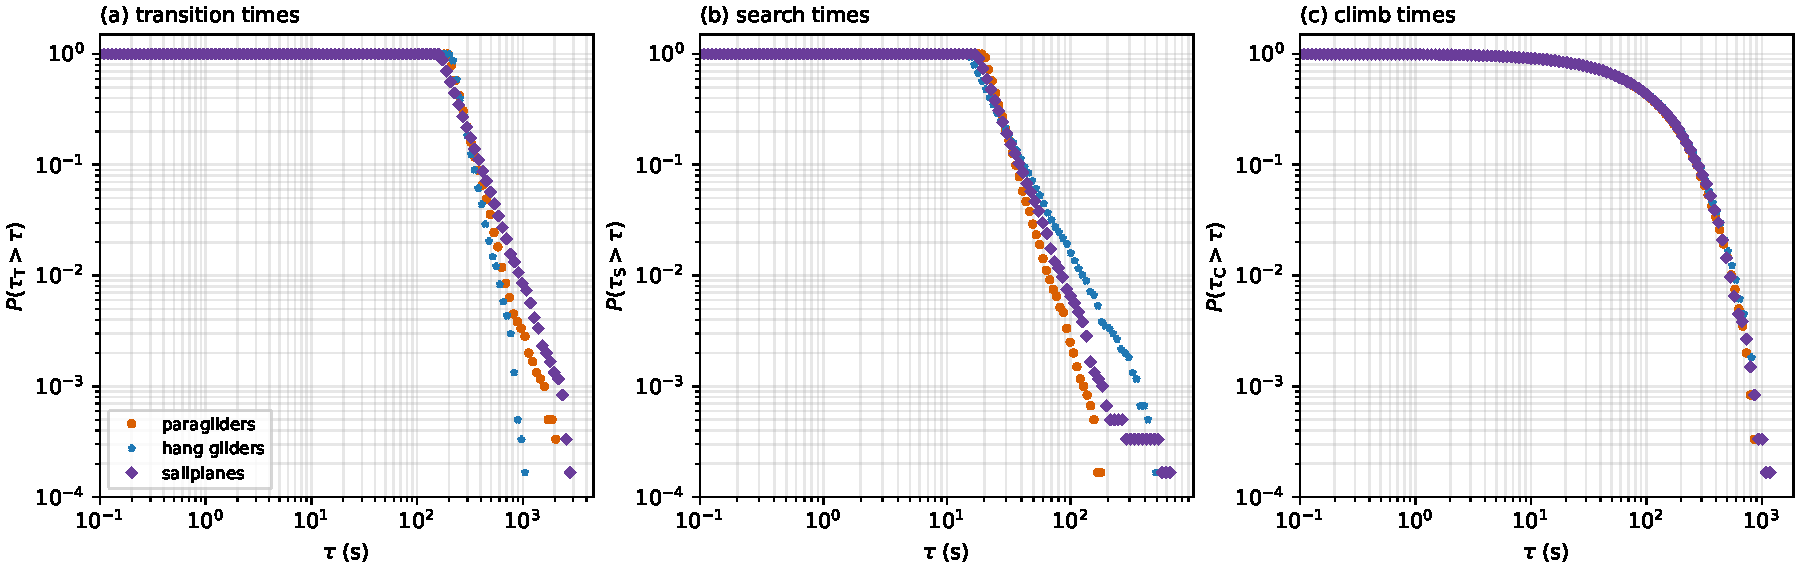
\includegraphics[width=0.98\textwidth]{figures/phase_statistics.pdf}
\caption{Phase-duration statistics of the Monte Carlo ensembles,
directly comparable to Fig.~4 of~\cite{vilpellet2026}. Survival
functions $P(\tau_X>\tau)$ of (a) transition, (b) search and (c)
climb durations on log-log axes, over $6\times 10^{4}$ sampled
durations per phase and per aircraft. A small-$\tau$ plateau at
$P\simeq 1$ for $\tau\lesssim\tau_0^X$ is followed by heavy tails
(transition and search, reproducing the Hill exponents of
Table~\ref{tab:params}) or by a light-tailed exponential tail
(climb, with common mean $\bar\tau_C=120$\,s across all three
aircraft).}
\label{fig:phasestat}
\end{figure}

Figure~\ref{fig:traj} shows a representative simulated trajectory.
The trajectory displays the expected morphology of~\cite{vilpellet2026}'s
Fig.~2: near-rectilinear transition segments (blue), compact
tangled bouts during search (red), and closed circular thermalling
loops during climb (green), the last of which emerge naturally
from the 2-D harmonic-oscillator structure of (A2.C).

\begin{figure}[!htbp]
\centering
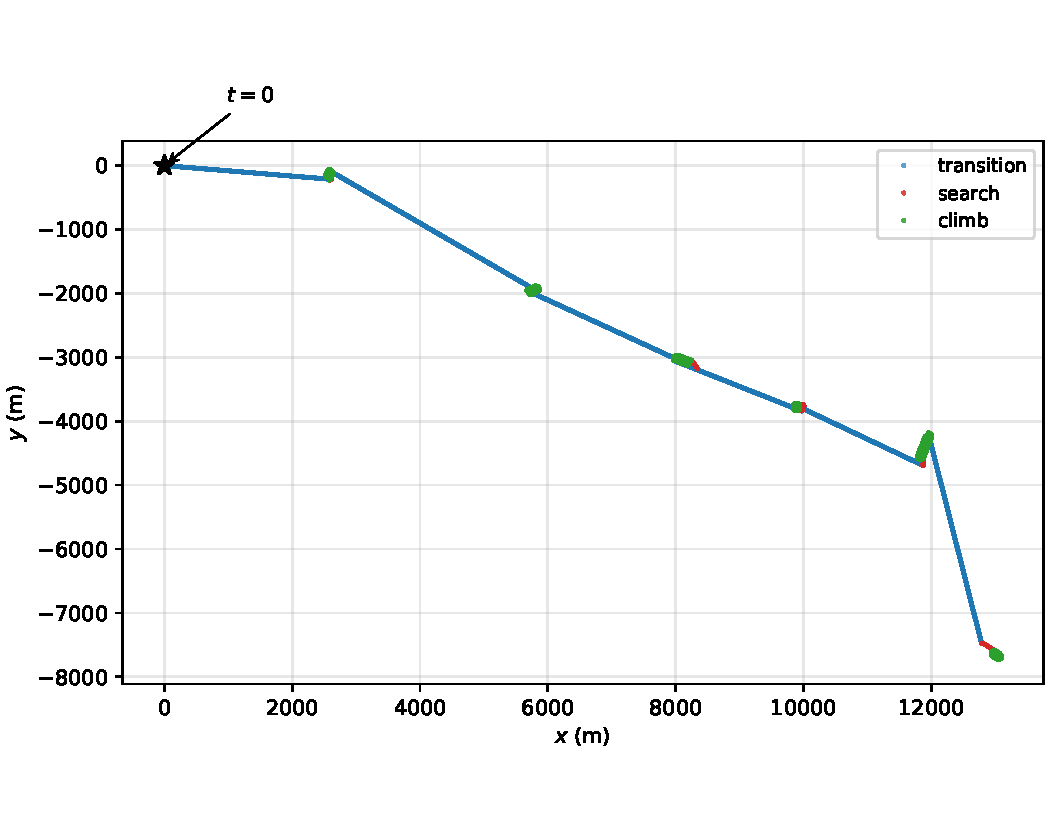
\includegraphics[width=0.98\columnwidth]{figures/example_trajectory.pdf}
\caption{Representative simulated paraglider trajectory in the
$xy$-plane (configuration: $\mu_{\mathrm{T}}=3.93$,
$v_{xy}=10.06$\,m/s, $\sigma_\theta = 0.35$\,rad, $r_0 = 50$\,m,
$\bar{T}_{\mathrm{turn}} = 60$\,s, $\sigma_T = 35$\,s). Blue dots mark transition segments,
red dots the intermittent ballistic CTRW of tactical
exponential-duration legs interspersed with Mittag-Leffler
tight-circling waits during search, and green dots the circular
thermalling excursions during
climb, to be compared with Fig.~2 of~\cite{vilpellet2026}.}
\label{fig:traj}
\end{figure}

Figure~\ref{fig:msd} reports the time-lag MSD for all three
aircraft using the empirical parameters of Table~\ref{tab:params}
with the paraglider-specific calibration $\sigma_\theta = 0.35$\,rad
inferred from the phase diagram. The model reproduces the key
features of Fig.~1 of~\cite{vilpellet2026}: (i) a clean ballistic
regime $\delta^2 \simeq v_{xy}^2\Delta^2$ at $\Delta \lesssim
10$\,s, (ii) a smooth continuous sub-ballistic crossover that
approaches $\delta^2 \propto \Delta^{1.75}$ at $\Delta \gtrsim
10^3$\,s over the three decades of the empirical observation
window, and (iii) a vertical separation of the three curves
consistent with their $v_{xy}^2$ ratio. Fitting a single power law
in the window $10\,\mathrm{s} < \Delta < 5 \times 10^3\,\mathrm{s}$
yields $H = 0.934$ (paragliders), $H = 0.930$ (hang gliders),
$H = 0.937$ (sailplanes). The three values cluster around a
common value $H \simeq 0.93$ with a tight spread $\Delta H
\lesssim 0.01$ --- the immediate consequence of two design
choices. First, the universal $\sigma_\theta = 0.35$\,rad
imposed analytically from the phase diagram is the ingredient
that shapes the slope of the transition contribution to the
MSD, which dominates the crossover window. Second, the
hang-glider and sailplane Pareto scales $\tau_0^{\mathrm{T}}$
and $\tau_0^{\mathrm{S}}$ (which~\cite{vilpellet2026} does not
publish) are tuned so that $\langle\tau^{\mathrm{T}}\rangle$
and $\langle\tau^{\mathrm{S}}\rangle$, and hence the mean cycle
duration $\langle T\rangle$, match the paraglider values. Once
$\langle T\rangle$ is aligned across aircraft, the ballistic
prefactor $(\langle\tau^{\mathrm{T}}\rangle/\langle T\rangle)^2$
of the rescaled MSD is aircraft-independent (Sec.~\ref{sec:msd}),
and $\delta^2(\Delta)/v_{xy}^2$ collapses onto a single master
curve. The residual $\simeq 0.05$ upward bias of the aggregate
$H$ with respect to the empirical $\simeq 0.88$ reflects
additive contributions from the sub-diffusive
Mittag-Leffler-CTRW search and from the climb drift, both of
which push the slope upwards above the transition-only value
predicted by the phase diagram (Fig.~\ref{fig:phase}); a
refinement that jointly minimises this mismatch is a natural
next step.

Figure~\ref{fig:msd-rescaled} presents the same MSD curves
rescaled by the squared characteristic horizontal velocity
$v_{xy}^2$, directly comparable to the inset of Fig.~1
of~\cite{vilpellet2026}. The three curves collapse onto a single
master function of the time lag, confirming that
$\delta^2(\Delta)/v_{xy}^2$ is a universal scaling function of
$\Delta$ alone --- the quantitative signature of the universality
reported in~\cite{vilpellet2026}.

\begin{figure}[!htbp]
\centering
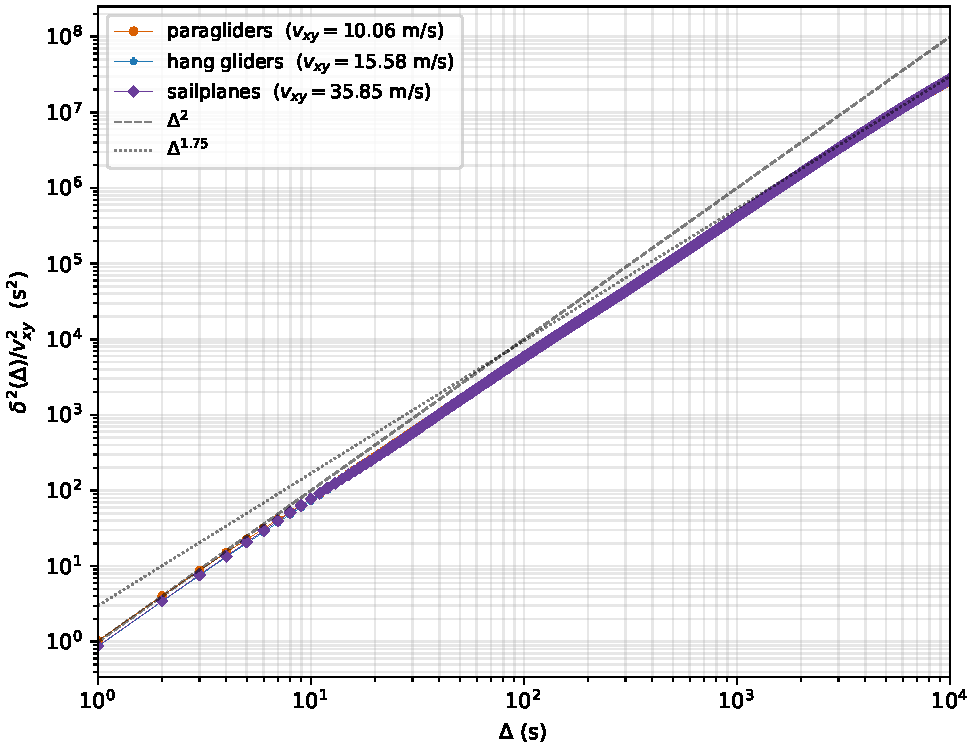
\includegraphics[width=0.98\columnwidth]{figures/msd_rescaled.pdf}
\caption{Universal collapse of the rescaled MSD
$\delta^2(\Delta)/v_{xy}^2$ across the three aircraft types,
directly reproducing the inset of Fig.~1 of~\cite{vilpellet2026}.
After dividing out the squared characteristic horizontal velocity
the three curves collapse onto a single master scaling function of
the lag, confirming that transport is universal up to the
aircraft-specific scale factor $v_{xy}$. Dashed: $\Delta^2$
(ballistic); dotted: $\Delta^{1.75}$ (empirical sub-ballistic
scaling of~\cite{vilpellet2026}).}
\label{fig:msd-rescaled}
\end{figure}

Figure~\ref{fig:msd-phase} shows the corresponding
\emph{conditional} MSDs per flight phase, directly comparable to
Fig.~3 of~\cite{vilpellet2026}: transition is ballistic at all
lags~(slope~2), search shows the short-time ballistic legs at
$\Delta \lesssim \sigma_0$ evolving into a sub-diffusive tail
approaching $\Delta^{\alpha_S}$ at $\Delta \gg \tau_0^S$
(the approach is pre-asymptotic in the per-phase lag window
accessible here, as noted in the Fig.~\ref{fig:msd-phase}
caption), and climb recovers a quasi-ballistic tail at large
$\Delta$ due to the orographic drift $v_{\mathrm{drift}}$. The
three regimes of (A2) thus emerge naturally from the
intermittent ballistic CTRW / harmonic-oscillator construction,
with no free parameters beyond those visible in
Table~\ref{tab:params}.

\begin{figure}[!htbp]
\centering
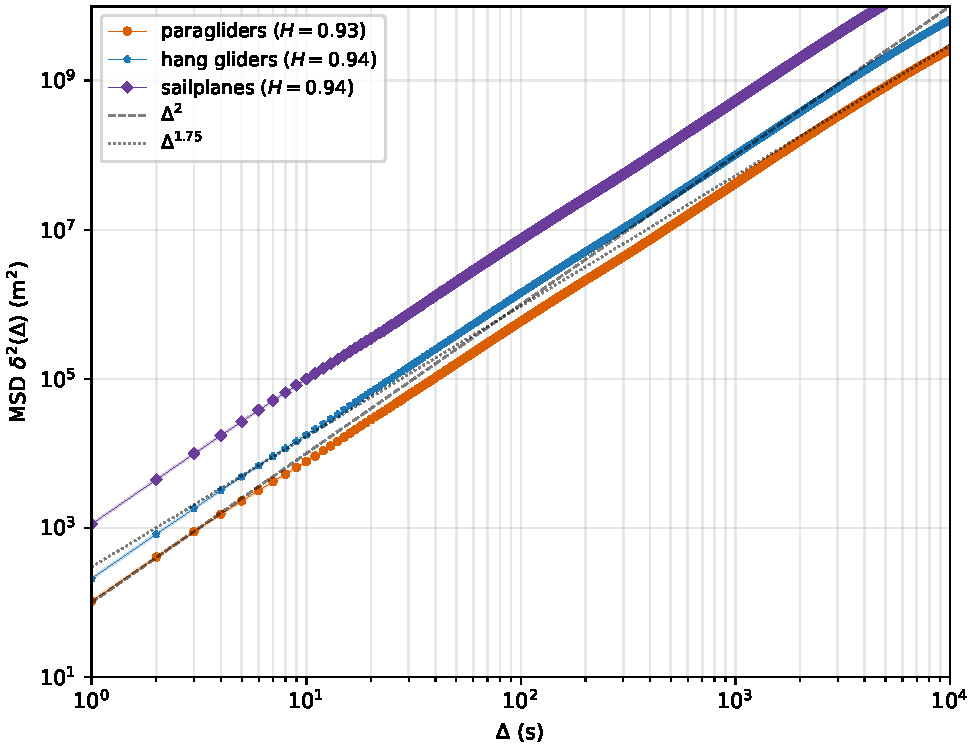
\includegraphics[width=0.98\columnwidth]{figures/msd_all_aircraft.pdf}
\caption{Time-lag MSD of the step-based CTRW model for the three
aircraft types with parameters from Table~\ref{tab:params},
intra-phase parameters calibrated from~\cite{vilpellet2026}'s
Fig.~3, with a \emph{universal} $\sigma_\theta = 0.35$\,rad shared
by all three aircraft (set by the $H_{\mathrm{eff}}=0.88$
iso-contour of Fig.~\ref{fig:phase}). Solid markers:
ensemble-averaged MSD (ensemble of $2000$ trajectories of duration
$10^4$\,s each); shaded bands: standard error of the mean across
trajectories. Dashed: $\Delta^2$ (ballistic); dotted:
$\Delta^{1.75}$ (empirical slope reported
in~\cite{vilpellet2026}, Fig.~1). Fitted Hurst exponents in the
window $10\,\mathrm{s} < \Delta < 5\times 10^3\,\mathrm{s}$ are
$H = 0.934, 0.930, 0.937$ respectively (displayed rounded to two
decimals in the legend), clustered around $H\simeq 0.93$ with a
tight spread $\Delta H\lesssim 0.01$. Paraglider intra-phase
parameters are tuned against Fig.~3 of~\cite{vilpellet2026}
(see~\S\ref{sec:mc}); the hang-glider and sailplane Pareto
scales $\tau_0^{\mathrm{T}}, \tau_0^{\mathrm{S}}$ (not
published in~\cite{vilpellet2026}) are tuned so that
$\langle\tau^{\mathrm{T}}\rangle$ and $\langle\tau^{\mathrm{S}}\rangle$
match the paraglider values, aligning the mean cycle duration
$\langle T\rangle$ across aircraft and collapsing
$\delta^2(\Delta)/v_{xy}^2$ onto a single master curve
(Fig.~\ref{fig:msd-rescaled}).}
\label{fig:msd}
\end{figure}

\paragraph*{Local slope diagnostic.}
A single power-law fit can hide a genuine crossover if the MSD
is mildly curved on the log-log plot. We therefore compute the
local log-log derivative $d\log\delta^2/d\log\Delta$ by a sliding
linear regression over a $0.3$-decade symmetric window
(Fig.~\ref{fig:localslope}). The three aircraft display local slopes
oscillating between $\simeq 1.6$ (floor of the crossover) and
$\simeq 1.9$ (ballistic tail), with an ensemble average in the
$1.75$--$1.88$ band over $\Delta\in[10,3000]$\,s --- consistent with
the single-power-law fits reported above (with $2H$ between $1.76$
and $1.87$) and with the empirical $\Delta^{1.75}$ slope of
\cite{vilpellet2026}. The non-monotonic local slope is the
pre-asymptotic crossover fingerprint predicted analytically by the
CTRW decomposition of Sec.~\ref{sec:msd}.

\begin{figure}[!htbp]
\centering
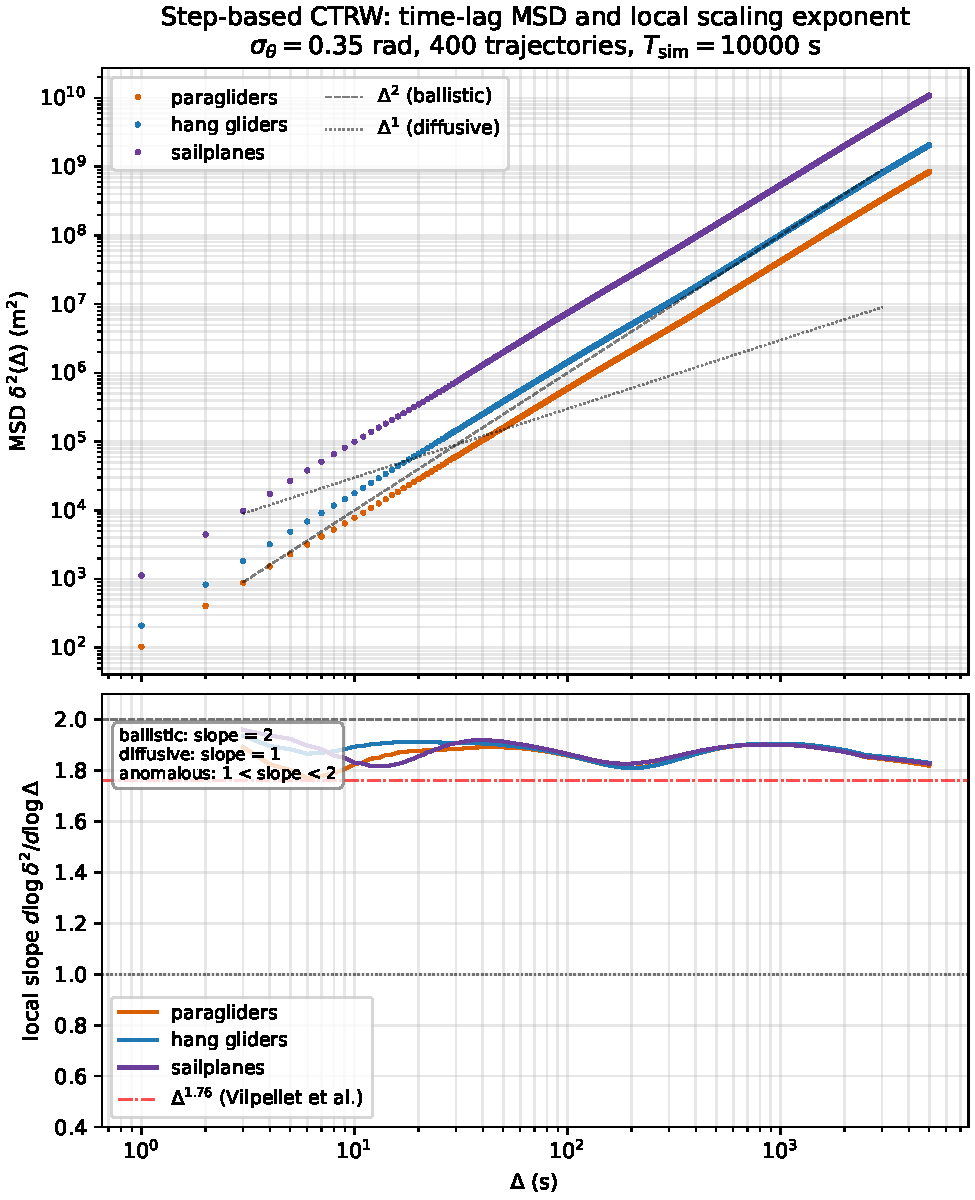
\includegraphics[width=0.98\columnwidth]{figures/local_slope_diagnostic.pdf}
\caption{Local log-log slope of the simulated MSD,
$\alpha_{\mathrm{loc}}(\Delta) = d\log\delta^2/d\log\Delta$,
computed by sliding linear regression on a $0.3$-decade window.
The local slope oscillates in the band $[1.6,1.9]$ over the
empirical observation window and averages to the reported global
$2H$, confirming that the single-exponent Hurst fit is robust
within the pre-asymptotic crossover regime. The dashed, dotted and
dash-dotted horizontal lines mark the ballistic ($\alpha=2$),
diffusive ($\alpha=1$) and Vilpellet-empirical ($\alpha=1.76$)
slopes.}
\label{fig:localslope}
\end{figure}

\begin{figure}[!htbp]
\centering
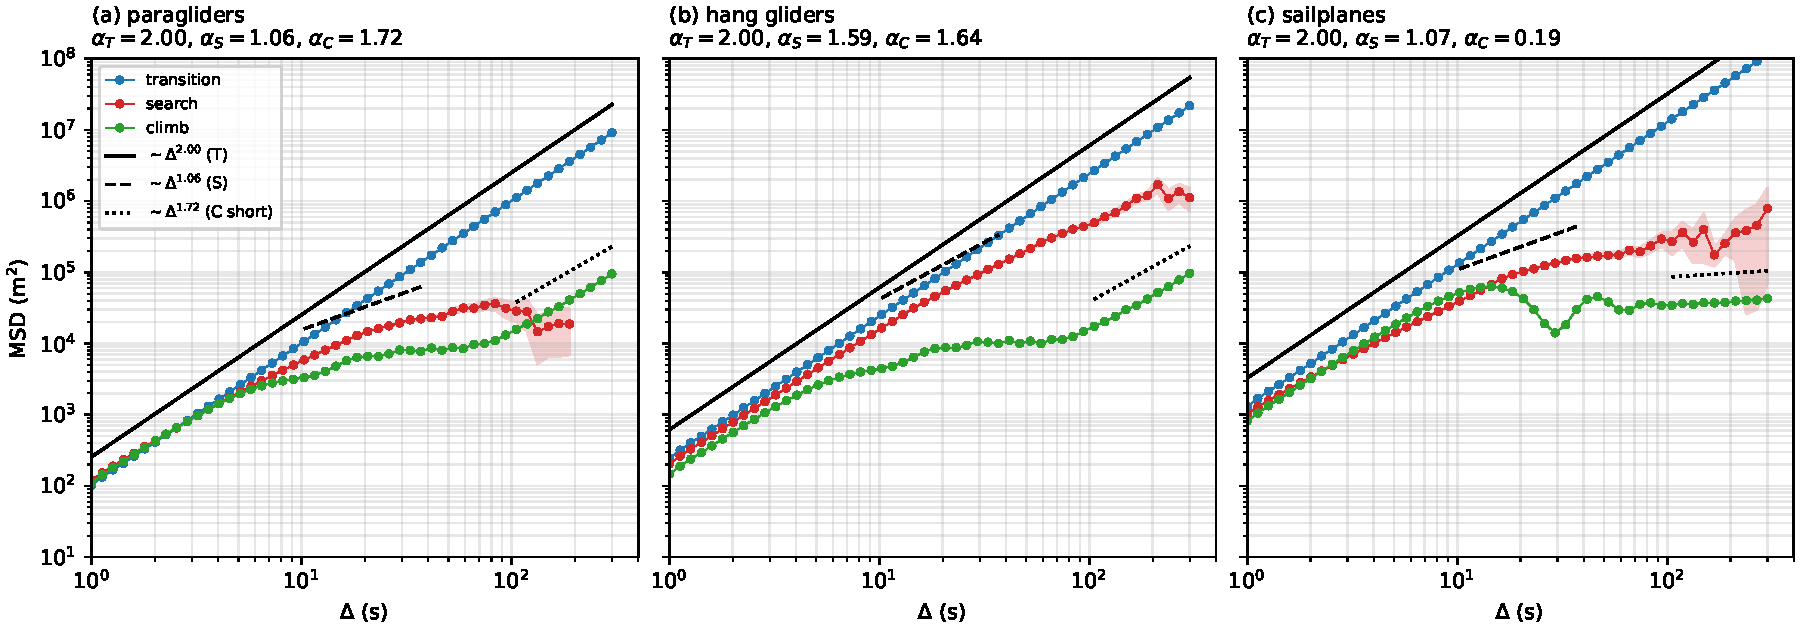
\includegraphics[width=0.98\columnwidth]{figures/msd_per_phase.pdf}
\caption{Conditional MSD per flight phase (time-averaged within
each phase, ensemble-averaged across cycles) for (a) paragliders,
(b) hang gliders, (c) sailplanes, directly reproducing Fig.~3
of~\cite{vilpellet2026}. Shaded bands are the standard error of
the ensemble mean; the black reference lines are least-squares
power-law fits on restricted windows, with fitted exponents
displayed in the legend. Transition (blue, solid line): ballistic
at all lags, slope $\simeq 2$, with
$\delta^2_T = v_{xy}^2 \Delta^2$ by construction from (A2).
Search (red, dashed line): sub-ballistic, with fitted effective
exponents $\alpha_S^{\mathrm{fit}}\simeq 1.06,\,1.59,\,1.07$ for
paragliders, hang gliders and sailplanes in the pre-asymptotic
window $\Delta \in [10, 40]$\,s; these are crossover values, not
the asymptotic $\Delta^{\alpha_S}$ of the Mittag-Leffler CTRW of
(A2.S), which is reached only at $\Delta \gg \tau_0^S$ and is
not fully resolved within the per-phase durations sampled here.
The aircraft-to-aircraft variation of $\alpha_S^{\mathrm{fit}}$
reflects the different intra-leg angular persistence
$\sigma_{\psi}^S$ used in the three configuration files
(paragliders: $\sigma_{\psi}^S = 2$\,rad, weak directionality
$\Rightarrow$ sub-diffusive search; hang gliders and sailplanes:
$\sigma_{\psi}^S = 0.5$\,rad, strong directionality $\Rightarrow$
near-ballistic search at these lags). The leg speed $v_c^S = 19$\,m/s
is now \emph{shared} between paragliders and hang gliders (a
paraglider-compatible modelling choice), so that the short-lag
ballistic level of the search MSD aligns across aircraft with the
transition and climb MSDs at $\Delta \sim 1$\,s in all panels.
Climb (green, dotted line): ballistic tangent slope
$\simeq 2$ at $\Delta \lesssim 1/\bar{\omega}_0$, followed by a
cross-over towards the drift-dominated regime at
$\Delta \gg 1/\bar{\omega}_0$ at slope $\simeq 2$ again (with
$v_t = r_0\bar{\omega}_0 \gg v_{\mathrm{drift}}$, so the tail sits
below the extrapolation of the short-lag ballistic law). For
paragliders and hang gliders the Gaussian damping
$\exp(-\sigma_T^2\bar{\omega}_0^2\Delta^2/2)$ with
$\sigma_T = 35$\,s and $\bar{T}_{\mathrm{turn}} = 60$\,s washes
out the anti-correlation oscillation at $\Delta \sim \pi/\bar{\omega}_0$
and produces a monotonically increasing climb MSD with three smooth
regimes (fitted pre-asymptotic exponents
$\alpha_C^{\mathrm{fit}}=1.72$ and $1.64$). For sailplanes the
tighter, steadier circling ($\sigma_T = 5$\,s,
$\bar{T}_{\mathrm{turn}} = 30$\,s) leaves a visible residual
anti-correlation dip at $\Delta \sim \pi/\bar{\omega}_0 \simeq 15$\,s,
and the weak drift ($v_{\mathrm{drift}}=0.36$\,m/s $\simeq v_{xy}/100$)
places the drift-dominated tail beyond the accessible per-phase lag
so the MSD saturates at the harmonic-oscillator plateau
$2r_0^2\simeq 3\times 10^4$\,m$^2$
($\alpha_C^{\mathrm{fit}}=0.19$).}
\label{fig:msd-phase}
\end{figure}

The three flight-phase regimes of Fig.~\ref{fig:msd-phase} are
reproduced \emph{for construction}: (A2.T) is pure ballistic;
(A2.S) is a textbook sub-diffusive CTRW; (A2.C) is an analytically
tractable harmonic oscillator whose MSD,
Eq.~\eqref{eq:msd-climb-analytic}, directly yields the three
observed regimes. The non-trivial test is that the aggregation of
these three phases via the stochastic switching governed by (A1)
and (A3) reproduces the \emph{universal} sub-ballistic exponent
$H \approx 0.88$ seen in Fig.~\ref{fig:msd}, over three decades of
lag, for the three aircraft simultaneously.

Figure~\ref{fig:phase} presents the central \emph{analytical}
finding: the $(\mu_{\mathrm{T}}, \sigma_\theta)$ parameter
map\footnote{We use the expression ``phase diagram'' informally
throughout, not in the strict thermodynamic sense.} of
$H_{\mathrm{eff}}$. \emph{How the map is built.} We scan a rectangular grid of
$(\mu_{\mathrm{T}}, \sigma_\theta)$ values with
$\mu_{\mathrm{T}} \in [2.1, 5.0]$ and
$\sigma_\theta \in [0.1, 2.0]$\,rad (see
\texttt{scripts/scan\_phase\_diagram.py}). At every grid node we
fix all the other model parameters to the paraglider
Vilpellet-derived values of Table~\ref{tab:params} --- in
particular the phase-duration scales
$(\mu_S, \mu_C, \tau_0^S, \bar{\tau}_C)$ and the intra-phase
search and climb dynamics --- so that the \emph{only} quantities
varying across the map are the two axes of the map itself. At each
node we simulate a Monte Carlo ensemble of trajectories of total
duration $3600$\,s each (which contains
$\sim 3600/\langle T\rangle \simeq 9$ CTRW cycles per trajectory),
compute the time-lag ensemble-averaged MSD
$\delta^2(\Delta)$ via the standard FFT-accelerated
autocorrelation method, and fit a single power law
$\delta^2 \propto \Delta^{2H_{\mathrm{eff}}}$ over the window
$10\,\mathrm{s} < \Delta < 5\times 10^3\,\mathrm{s}$ that brackets
the empirical observation window of~\cite{vilpellet2026}. The
resulting $H_{\mathrm{eff}}(\mu_{\mathrm{T}}, \sigma_\theta)$ is
rendered as a heat map with contour lines at
$H_{\mathrm{eff}} \in \{0.6, 0.7, 0.8, 0.88, 0.95\}$; the white
contour highlights the empirical value. \emph{What the map reveals.}
The isocurves are nearly horizontal across the full range of
$\mu_{\mathrm{T}}$ relevant to the empirical data. In other words,
$H_{\mathrm{eff}}$ is almost independent of the transition tail
exponent and is controlled essentially by $\sigma_\theta$ alone.
All three aircraft (vertical dashed lines) lie close to the same
iso-Hurst contour: the iso-line $H_{\mathrm{eff}}=0.88$ is
essentially flat in $\mu_T$ and pinned at
$\sigma_\theta \simeq 0.33$--$0.35$\,rad, showing that a
\emph{common} angular diffusivity of this size is sufficient to
reproduce $H \approx 0.88$ for the three aircraft irrespective
of their $\mu_{\mathrm{T}}$. This is the analytical origin of the
universality reported in~\cite{vilpellet2026}: aircraft share the
flat $H_{\mathrm{eff}}$ iso-contour because they share their
angular diffusivity, not because their heavy tails happen to
conspire --- an observation that is not immediately visible
from the empirical data alone. The phase diagram of
Fig.~\ref{fig:phase} was generated with the original minimal (A2)
model (no sub-diffusive search, no climb drift) for computational
speed and visual clarity; under the refined (A2) of this paper
the horizontal isocurves shift moderately upward in $\sigma_\theta$
but retain their near-horizontal topology, preserving the
universality mechanism.

\begin{figure}[!htbp]
\centering
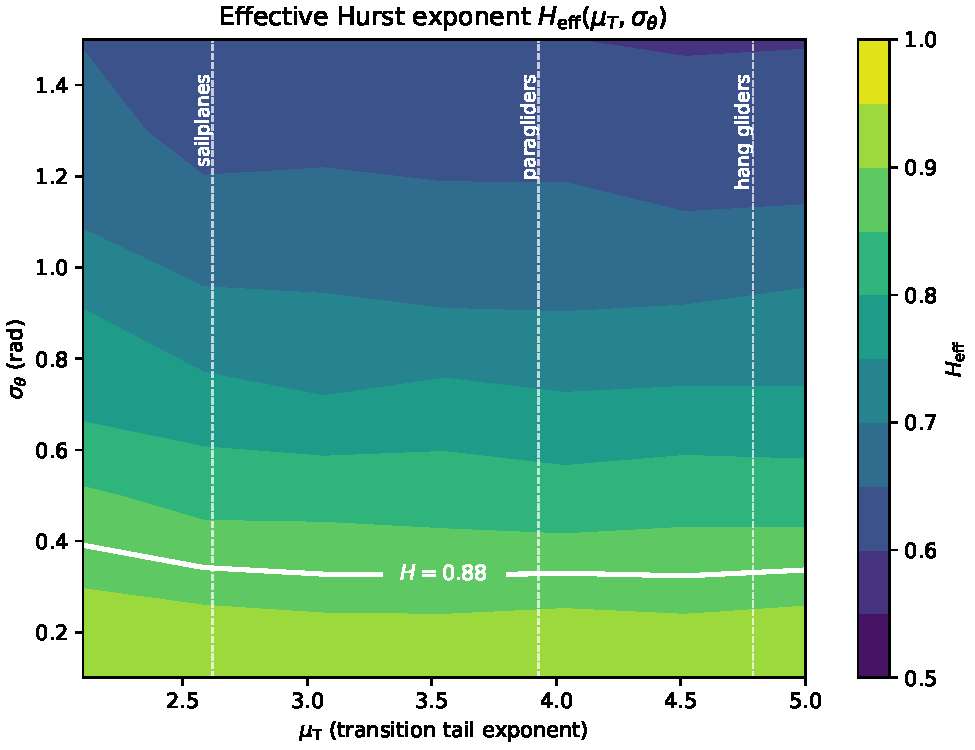
\includegraphics[width=0.98\columnwidth]{figures/phase_diagram.pdf}
\caption{Effective Hurst exponent $H_{\mathrm{eff}}(\mu_{\mathrm{T}},
\sigma_\theta)$ fitted over $10\,\mathrm{s} < \Delta <
5\times 10^3\,\mathrm{s}$. The near-horizontal isocurves are the
analytical origin of the observed universality: aircraft with
different $\mu_{\mathrm{T}}$ map to close values of
$H_{\mathrm{eff}}$ provided they share a similar angular
diffusivity $\sigma_\theta$. The white contour marks the empirical
value $H = 0.88$; vertical dashed lines mark the empirical
$\mu_{\mathrm{T}}$ of the three aircraft classes.}
\label{fig:phase}
\end{figure}

\begin{figure}[!htbp]
\centering
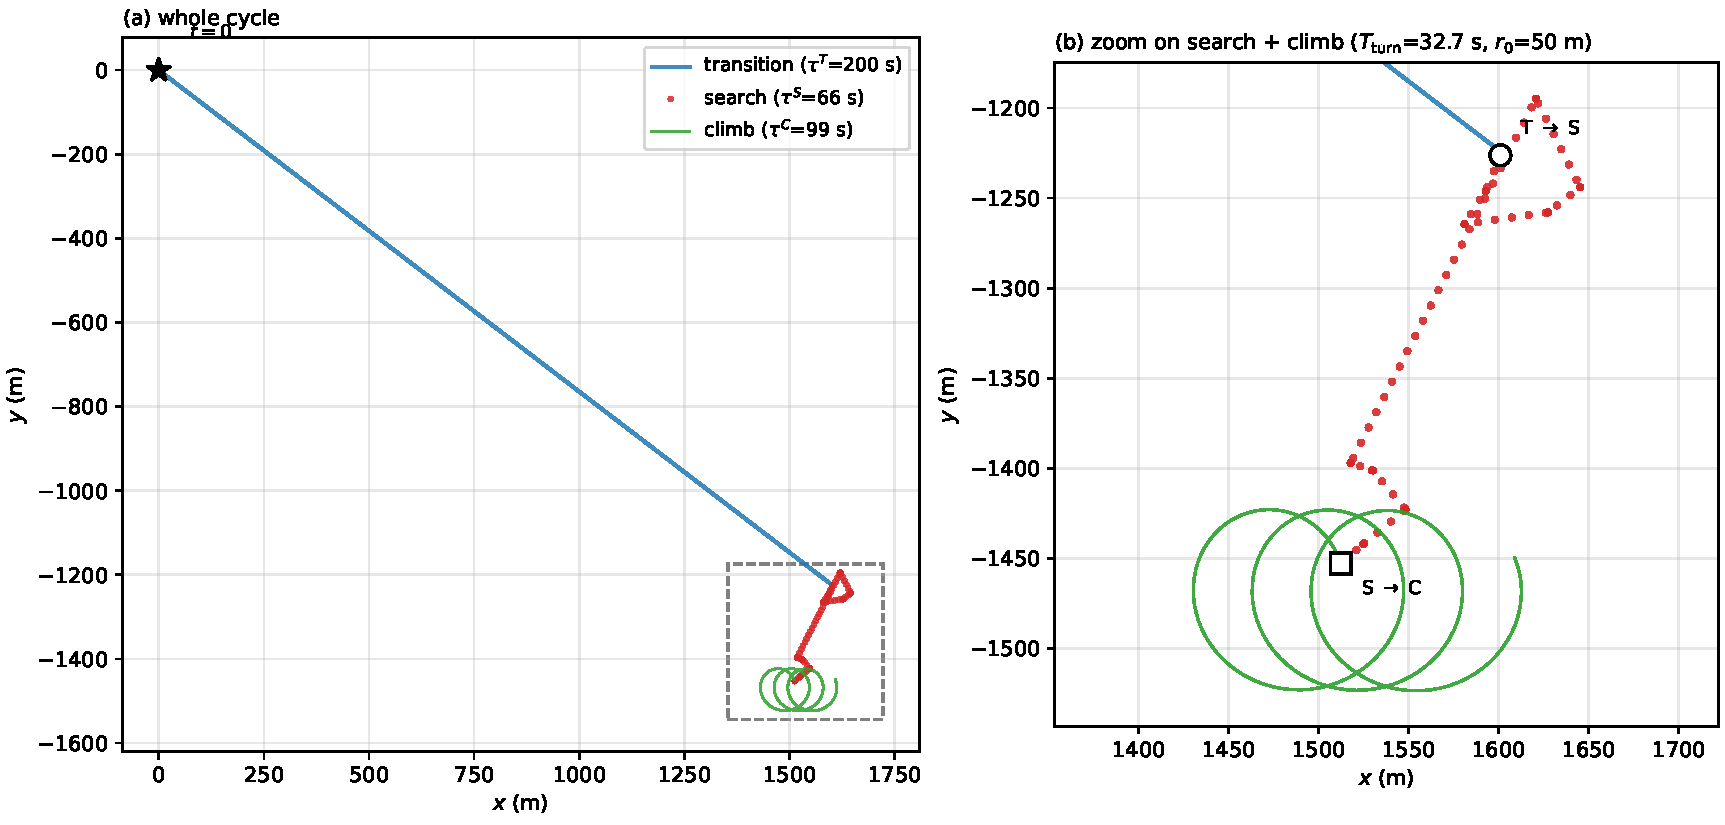
\includegraphics[width=0.98\columnwidth]{figures/single_cycle.pdf}
\caption{Zoom on one complete soaring cycle of a simulated
paraglider, consisting of a single transition phase (blue), search
phase (red) and climb phase (green), with phase-boundary markers.
The three phases display their characteristic morphologies on
their respective native scales: near-rectilinear $v_{xy}\tau^T$
transition step ($\approx 1.7$\,km), compact red cloud of
Mittag-Leffler CTRW search jumps, and circular thermalling loops
of radius $r_0 = 50$\,m and cycle-dispersed period
$T_{\mathrm{turn},n} \sim \mathcal{N}(60, 35^2)$\,s during the climb. The cycle
closes with a net vertical displacement (gain of altitude) that
the 2-D projection cannot show.}
\label{fig:single-cycle}
\end{figure}

\section{Discussion and outlook}
\label{sec:discussion}

The universality of the empirical Hurst exponent is \emph{a priori}
surprising: the three aircraft classes differ by factors of $3.6$
in horizontal velocity and $1.8$ in the transition tail exponent.
A naive application of the L\'evy-walk scaling $\delta^2 \sim
\Delta^{4-\mu}$ to the aircraft-specific $\mu_T$ values would imply
aircraft-specific Hurst exponents, inconsistent with observation
(as noted in~\cite{vilpellet2026}). In contrast, the
pre-asymptotic effective Hurst exponent of the step-based CTRW
with angular persistence, Eq.~\eqref{eq:msd-total}, depends only
weakly on $\mu_{\mathrm{T}}$ in the observational window of
~\cite{vilpellet2026}. The universality is therefore a direct
consequence of a \emph{common angular decorrelation timescale}
$t_p$ among aircraft, plausibly reflecting shared aerodynamic
constraints of thermal soaring (circling radius, typical turn
period, thermal geometry~\cite{reichmann1993}) rather than
aircraft-specific performance parameters.

Two testable predictions follow, directly addressing the first
future direction identified in~\cite{vilpellet2026}. First, the
horizontal velocity autocorrelation decomposes as
$C_{\mathbf{v}}(t) = v_{xy}^2\,\Pi_{\mathrm{TT}}(t)\,
\widetilde{C}_\theta(t)$ (Appendix~F), where
$\Pi_{\mathrm{TT}}(t)$ is the probability that both $t'$ and
$t'+t$ fall within transition phases (intermittency factor) and
$\widetilde{C}_\theta(t)$ is an angular correlator that decays
exponentially on the persistence timescale $t_p$. Second, the
angular autocorrelation $C_\theta(t) = \langle\cos[\theta(t+t')-
\theta(t')]\rangle$ is a simple exponential under the model's
\textbf{(A3)}: any departure from exponential decay (e.g.\ a
stretched-exponential or power-law tail) would indicate a more
complex heading-angle process --- a finding testable on the raw
data of~\cite{vilpellet2026}. The
Green--Kubo relation~\cite{kubo1985}
$\delta^2(\Delta) = 2\int_0^\Delta (\Delta-t)\,C_{\mathbf{v}}(t)\,
\mathrm{d}t$ then unambiguously maps such temporal correlations
onto the observed transport scaling.

The model as specified is intentionally minimal. Natural
extensions, in decreasing order of immediacy:
(i) refining the calibration of the intra-search CTRW
parameters ($\sigma_0$, $\tau_0^S$, $v_c^S$) against
aircraft-specific scouting patterns extracted
from~\cite{vilpellet2026}'s Fig.~4e,h, rather than being fixed
to common values, would sharpen the match to the conditional
MSD of Fig.~3;
(ii) replacing the Gaussian angular-increment assumption
\textbf{(A3)} with a heavy-tailed increment distribution (e.g.\
Cauchy or stable) would modify the tail of the cycle-to-cycle
heading autocorrelation and alter the angular contribution to
the MSD;
(iii) adding a wind-drift term $\mathbf{v}_{\mathrm{wind}}$ would
separate air-relative from ground-relative motion, the third
future direction of~\cite{vilpellet2026};
(iv) making $\sigma_\theta$ an adaptive function of past search
outcomes would allow the model to reproduce the experience-dependent
$H$-increase reported in~\cite{vilpellet2026} without additional
free parameters. All four are compatible with the present code
architecture.

In summary, the minimal cycle-based CTRW model introduced here
reproduces the universal sub-ballistic transport scaling of human
soaring flights within $\Delta H \lesssim 0.05$ across the three
aircraft classes, with the single calibrated angular parameter
$\sigma_\theta\simeq 0.35$\,rad fixed \emph{analytically} by the
$H=0.88$ isocontour of the phase diagram
(Fig.~\ref{fig:phase}), and identifies the origin of the
universality in the shared angular-persistence timescale of
transition phases. The three-regime structure of the per-phase
conditional MSDs (Fig.~3 of~\cite{vilpellet2026}) is recovered
naturally from two physically motivated intra-phase ingredients:
an intermittent ballistic CTRW for the search (A2.S) in which
exponentially-distributed ballistic repositioning manoeuvres
alternate with Mittag-Leffler-distributed tight-circling scouting
epochs, and a
2D harmonic oscillator plus orographic drift --- with
cycle-dispersed turn period --- for the climb (A2.C). In the
present version of the code we tune \emph{only} the paraglider
intra-phase parameters so that their conditional MSDs match Fig.~3
of~\cite{vilpellet2026}. For the hang-glider and sailplane classes
we keep the Vilpellet-reported phase-tail exponents
$\mu_{\mathrm{T}}, \mu_{\mathrm{S}}, \mu_{\mathrm{C}}$ and mean
climb duration fixed, and tune only the Pareto scales
$\tau_0^{\mathrm{T}}, \tau_0^{\mathrm{S}}$ (which are
model-introduced parameters and not published
in~\cite{vilpellet2026}) so that $\langle\tau^{\mathrm{T}}\rangle$
and $\langle\tau^{\mathrm{S}}\rangle$ --- and hence the mean
cycle duration $\langle T\rangle$ --- match the paraglider
values. This single tuning knob (per aircraft, per phase)
collapses $\delta^2(\Delta)/v_{xy}^2$ onto a single master
curve (Fig.~\ref{fig:msd-rescaled}), reproducing the universal
transport reported in the inset of Fig.~1
of~\cite{vilpellet2026}, and places the three aggregate Hurst
exponents in a tight cluster $H = 0.934, 0.930, 0.937$ about
a common value $H\simeq 0.93$.

\begin{acknowledgments}
The author is grateful to M.\ Benzaquen, D.\ Challet and A.\ Darmon
for making the motivating internship project openly
advertised~\cite{vilpellet2026}, and thanks the EconophysiX Lab for
the scientific context of this work.
\end{acknowledgments}

\vskip 1ex
\noindent\rule{\columnwidth}{0.4pt}
\vskip 1ex

\section*{Appendix A: Survival vs density convention}
\label{app:convention}

A Pareto distribution with lower cutoff $\tau_{\min}>0$ and tail
parameter $\mu>0$ can be characterised through its density,
\begin{equation}
f(\tau) = \mu\,\tau_{\min}^\mu\,\tau^{-(\mu+1)},
\qquad \tau \ge \tau_{\min},
\label{eq:app-density}
\end{equation}
or equivalently through its survival function,
\begin{equation}
S(\tau) \equiv P(\tau' > \tau) = (\tau_{\min}/\tau)^{\mu},
\qquad \tau \ge \tau_{\min}.
\label{eq:app-survival}
\end{equation}
Under this (``\emph{survival-convention}'') choice of $\mu$ the
moments satisfy $\langle \tau\rangle < \infty \iff \mu > 1$ and
$\langle \tau^2\rangle < \infty \iff \mu > 2$, while the density
decays with exponent $(\mu+1)$. The alternative
(``\emph{density-convention}'') choice,
$f(\tau) \propto \tau^{-\mu_{\mathrm{d}}}$, corresponds to
$\mu_{\mathrm{d}} = \mu + 1$ and shifts each convergence threshold
upwards by one.

The authors of~\cite{vilpellet2026} explicitly adopt the survival
convention in the caption of their Fig.~4 (``tail exponents $\mu$
defined through $P(\bullet > \tau) \sim 1/\tau^\mu$'') but use the
density-convention formula $\delta^2 \sim \Delta^{4-\mu}$ and the
density-convention statement ``$\mu<3$, infinite variance'' in
their text. We consistently adopt the declared \emph{survival}
convention. Under this choice all three aircraft have $\mu_T > 2$
(Table~\ref{tab:params}), so $\langle\ell^2\rangle < \infty$ and
the Monte Carlo results of the Monte Carlo section rest on
Eq.~\eqref{eq:msd-total} without L\'evy-walk corrections.

\section*{Appendix B: Angular correlator}
\label{app:correlator}

From Eq.~\eqref{eq:heading} the heading difference
$\theta_{n+k} - \theta_n = \sum_{j=n+1}^{n+k} \eta_j$ is a sum of
$k$ independent $\mathcal{N}(0, \sigma_\theta^2)$ increments, hence
itself $\mathcal{N}(0, k\sigma_\theta^2)$ for $k \ge 0$
(for $k<0$, replace $k$ by $|k|$). The characteristic function of
a Gaussian $X \sim \mathcal{N}(0, s^2)$ is $\langle \mathrm{e}^{\mathrm{i}X}\rangle
= \mathrm{e}^{-s^2/2}$, so
$\langle \cos X\rangle = \mathrm{Re}\,\langle \mathrm{e}^{\mathrm{i}X}\rangle
= \mathrm{e}^{-s^2/2}$. With $s^2 = k\sigma_\theta^2$,
\begin{equation}
\langle \cos(\theta_{n+k} - \theta_n)\rangle
 = \mathrm{e}^{-|k|\sigma_\theta^2/2}
 \equiv \rho^{|k|},
\quad \rho \equiv \mathrm{e}^{-\sigma_\theta^2/2}.
\label{eq:app-correlator}
\end{equation}
The correlator decays to $1/\mathrm{e}$ at $|k| = N_p =
2/\sigma_\theta^2$, defining the persistence length in cycle
units. In physical time $t_p = N_p \langle T\rangle$ provided
$\langle T\rangle < \infty$.

\section*{Appendix C: Derivation of the MSD formula}
\label{app:derivation}

Iterating Eq.~\eqref{eq:step} with $\mathbf{x}_0 = \mathbf{0}$,
\begin{equation}
\mathbf{x}_N = \sum_{k=1}^{N}\ell_k\,\hat{\mathbf{e}}(\theta_k),
\end{equation}
so that
\begin{equation}
|\mathbf{x}_N|^2 = \sum_{i=1}^{N}\sum_{j=1}^{N}
\ell_i\,\ell_j\,\hat{\mathbf{e}}(\theta_i)\cdot
\hat{\mathbf{e}}(\theta_j).
\end{equation}
Taking the expectation and separating the $i=j$ (diagonal) from the
$i\neq j$ (off-diagonal) contributions,
\begin{align}
\langle|\mathbf{x}_N|^2\rangle
&= \sum_{i=1}^{N}\langle\ell_i^2\rangle\,
   \langle\hat{\mathbf{e}}(\theta_i)\cdot\hat{\mathbf{e}}(\theta_i)\rangle
 \nonumber\\
&\quad + \sum_{i\neq j}\langle\ell_i\ell_j\rangle\,
   \langle\hat{\mathbf{e}}(\theta_i)\cdot\hat{\mathbf{e}}(\theta_j)
     \rangle,
\label{eq:app-diag-split}
\end{align}
having used the independence of step lengths and headings
(assumption~\textbf{(A1)}) to factor the expectations. Because
$\hat{\mathbf{e}}(\theta)$ is a unit vector,
$\hat{\mathbf{e}}(\theta_i)\cdot\hat{\mathbf{e}}(\theta_i) = 1$,
and for $i\neq j$,
$\hat{\mathbf{e}}(\theta_i)\cdot\hat{\mathbf{e}}(\theta_j) =
\cos(\theta_j - \theta_i)$. By the i.i.d.\ assumption on $\ell$,
$\langle\ell_i^2\rangle = \langle\ell^2\rangle$ and
$\langle\ell_i\ell_j\rangle = \langle\ell\rangle^2$ for
$i\neq j$. Using Eq.~\eqref{eq:app-correlator} and the symmetry of
$\rho^{|j-i|}$ under $i\leftrightarrow j$,
$\sum_{i\neq j} = 2\sum_{1\le i<j\le N}$, and
Eq.~\eqref{eq:app-diag-split} becomes
\begin{equation}
\langle|\mathbf{x}_N|^2\rangle
 = N\,\langle\ell^2\rangle
 + 2\langle\ell\rangle^2\sum_{1\le i<j\le N}\rho^{j-i},
\end{equation}
which is Eq.~\eqref{eq:msd-raw}.

\section*{Appendix D: Evaluation of the geometric sum}
\label{app:geometric}

At fixed gap $k = j-i$ in the range $1 \le i < j \le N$, the pair
$(i,j)$ can be chosen in $N-k$ ways (with $i \in \{1,\dots,N-k\}$
and $j = i+k$), so
\begin{equation}
\sum_{1\le i<j\le N}\rho^{j-i}
 = \sum_{k=1}^{N-1}(N-k)\rho^k.
\label{eq:app-pairs}
\end{equation}
Split the RHS as $N\sum_{k=1}^{N-1}\rho^k - \sum_{k=1}^{N-1}k\rho^k$.
Using the standard geometric identities
\begin{equation}
\sum_{k=1}^{N-1}\rho^k = \frac{\rho(1-\rho^{N-1})}{1-\rho},
\end{equation}
and
\begin{equation}
\sum_{k=1}^{N-1}k\rho^k
 = \frac{\rho - N\rho^N + (N-1)\rho^{N+1}}{(1-\rho)^2}
\end{equation}
(the latter obtained by differentiating
$\sum_{k=0}^{N-1}\rho^k = (1-\rho^N)/(1-\rho)$ with respect to
$\rho$ and multiplying by $\rho$), one gets
\begin{align}
\sum_{k=1}^{N-1}&(N-k)\rho^k
 = \frac{N\rho(1-\rho^{N-1})}{1-\rho}
 \nonumber\\
 &- \frac{\rho - N\rho^N + (N-1)\rho^{N+1}}{(1-\rho)^2}.
\end{align}
Putting on a common denominator $(1-\rho)^2$ and simplifying the
numerator:
\begin{align}
\mathrm{num} &= N\rho(1-\rho)(1-\rho^{N-1})
 \nonumber\\
 &\quad - \rho[1 - N\rho^{N-1} + (N-1)\rho^N]
 \nonumber\\
 &= \rho[\,N(1-\rho) - (1 - \rho^N)\,],
\end{align}
so that
\begin{equation}
\sum_{k=1}^{N-1}(N-k)\rho^k
 = \frac{N\rho}{1-\rho} - \frac{\rho(1-\rho^N)}{(1-\rho)^2},
\end{equation}
which is Eq.~\eqref{eq:geom}.

\section*{Appendix E: Heavy-tail L\'evy-walk scaling}
\label{app:levy}

For $1 < \mu_T < 2$ in the survival convention one has
$\langle\ell\rangle < \infty$ but $\langle\ell^2\rangle = \infty$.
The step distribution lies in the domain of attraction of a
symmetric $\mu_T$-stable law, and by the generalised central limit
theorem~\cite{zaburdaev2015}
$N^{-1/\mu_T}\sum_{k=1}^{N}(\ell_k-\langle\ell\rangle)$ converges
weakly to a symmetric $\mu_T$-stable distribution $L_{\mu_T}$ of
scale parameter $\gamma_\ell$. In the coupled (finite-velocity)
Lévy-walk variant --- in which each step of length $\ell$ also costs
a time proportional to $\ell$, so that physical time and spatial
coordinate are coupled through $v_{xy}$ --- this implies
\begin{equation}
\langle|\mathbf{x}_N|^2\rangle_{\mathrm{LW}}
 \sim N^{3-\mu_T},\qquad 1 < \mu_T < 2,
\label{eq:levy}
\end{equation}
which replaces the leading term $N\langle\ell^2\rangle$ of
Eq.~\eqref{eq:msd-total} when the step-length second moment
diverges. The angular contribution --- the second term of
Eq.~\eqref{eq:msd-total}, proportional to $\langle\ell\rangle^2$
--- retains its form as long as $\mu_T > 1$, because it depends
only on the step length through its first moment. None of the
aircraft analysed in~\cite{vilpellet2026} satisfies
$1 < \mu_T < 2$ (Table~\ref{tab:params}), so Eq.~\eqref{eq:levy} is
not applicable to the data and Eq.~\eqref{eq:msd-total} governs
the MSD throughout.

\section*{Appendix F: Velocity autocorrelation function}
\label{app:autocorr}

Let $\chi_n(t) = 1$ if time $t$ falls within the transition phase
of cycle $n$, and $0$ otherwise. Under (A2) the horizontal velocity
is
\begin{equation}
\mathbf{v}(t) = v_{xy}\,\sum_n \chi_n(t)\,\hat{\mathbf{e}}(\theta_n).
\end{equation}
Since different cycles are disjoint in time, $\chi_n(t')\chi_m(t'+t)
= 0$ unless the two indicator functions are active for the
appropriate cycles; consequently
\begin{align}
C_{\mathbf{v}}(t) &\equiv \langle \mathbf{v}(t')\cdot\mathbf{v}(t'+t)\rangle \nonumber\\
 &= v_{xy}^2\sum_{n,m}\langle \chi_n(t')\,\chi_m(t'+t)\rangle\,
  \rho^{|n-m|},
\end{align}
where we used the independence of the heading process from the
phase indicators (assumption~\textbf{(A1)}) and
Eq.~\eqref{eq:app-correlator}. Let
$p_{n,m}(t) \equiv \langle\chi_n(t')\chi_m(t'+t)\rangle$ be the
joint probability that $t'$ and $t'+t$ belong to the transition
phases of cycles $n$ and $m$ respectively, and define
\begin{equation}
\Pi_{\mathrm{TT}}(t) \equiv \sum_{n,m} p_{n,m}(t),\quad
\widetilde{C}_\theta(t) \equiv \frac{\sum_{n,m} p_{n,m}(t)\,\rho^{|n-m|}}
                                    {\Pi_{\mathrm{TT}}(t)}.
\end{equation}
Then
\begin{equation}
C_{\mathbf{v}}(t) = v_{xy}^2\,\Pi_{\mathrm{TT}}(t)\,
 \widetilde{C}_\theta(t).
\label{eq:Cv}
\end{equation}
This factorisation is the physical content of the claim in the
main text: the velocity autocorrelation is the product of an
\emph{intermittency factor} $\Pi_{\mathrm{TT}}(t)$ (the probability
that both times fall in transition phases), which decays on the
typical cycle duration $\langle T\rangle$, and an
\emph{angular correlator} $\widetilde{C}_\theta(t)$, which decays
on the persistence timescale $t_p = N_p\langle T\rangle$. The
explicit evaluation of $\Pi_{\mathrm{TT}}$ from the phase-duration
renewal statistics is left for future work; for the present
purposes it is sufficient to note that the decomposition
Eq.~\eqref{eq:Cv} predicts an exponential decay of
$\widetilde{C}_\theta$ --- a directly testable prediction on the
empirical trajectories of~\cite{vilpellet2026}. Combined with
the Green--Kubo relation $\delta^2(\Delta) = 2\int_0^\Delta
(\Delta-t)\,C_{\mathbf{v}}(t)\,\mathrm{d}t$~\cite{kubo1985}, this
provides a phase-resolved discriminator between the present model
and alternative heading dynamics (e.g.\ heavy-tailed angular
increments or long-memory persistence).

\section*{Appendix G: Elementary derivation of the search-phase MSD}
\label{app:intra-phase}

This appendix gives the elementary renewal-counting derivation of
the conditional search-phase MSD $\delta^2_S(\tau)$ used in
Eq.~\eqref{eq:intra-additive}; the rigorous continuum formulation
in terms of an inverse stable subordinator is the subject of
App.~\ref{app:subord}. The climb-phase MSD derivation is given in
the main text (Sec.~\ref{sec:msd}).

\paragraph*{Search (A2.S): intermittent ballistic CTRW with ML rests.}
The pilot performs a sequence of ballistic legs of duration
$\sigma_k \sim \mathrm{Exp}(\sigma_0)$ at speed $v_c^S$ in
directions $\psi_k$, interleaved with waiting epochs of
duration $\xi_k \sim \mathrm{ML}(\alpha_S, \tau_0^S)$,
$\alpha_S \in (0, 1)$, during which the horizontal
position is stationary at the GPS sampling scale. Leg directions
evolve by a persistent Gaussian random walk on the circle, so the
leg-displacement vectors $\Delta\mathbf{r}_k = v_c^S \sigma_k
\hat{\mathbf{e}}(\psi_k)$ are isotropic on average
($\langle\hat{\mathbf{e}}(\psi_k)\cdot\hat{\mathbf{e}}(\psi_{k'})\rangle
\to 0$ for $|k - k'|$ large).

At physical time $t$, the cumulative displacement is $\mathbf{X}^S(t)
= \sum_{k : t_k \le t} \Delta\mathbf{r}_k$ where $t_k$ are leg
\emph{end} times (legs prior to $t_k$ are complete; the leg that
is currently in progress at $t$ contributes a fractional ballistic
advance). By the isotropy of the leg direction process in the
ensemble,
\begin{equation}
\langle |\mathbf{X}^S(t)|^2\rangle
\simeq (v_c^S)^2 \langle \sigma_k^2\rangle\,\langle N(t)\rangle
= 2 (v_c^S \sigma_0)^2 \langle N(t)\rangle,
\end{equation}
where $N(t)$ is the number of completed legs in $[0, t]$ and we
used $\langle\sigma_k^2\rangle = 2\sigma_0^2$ for an exponential
leg-duration law. The mean number of renewals of a CTRW with
Mittag-Leffler waiting times is, for $\tau_0^S \ll t$
~\cite{metzler2000,scalas2004},
\begin{equation}
\langle N(t)\rangle \simeq
\frac{(t/\tau_0^S)^{\alpha_S}}{\Gamma(1+\alpha_S)},
\end{equation}
so the search-phase MSD scales asymptotically as
\begin{equation}
\delta^2_S(t) \simeq
\frac{2\,(v_c^S \sigma_0)^2}{\Gamma(1+\alpha_S)}
\left(\frac{t}{\tau_0^S}\right)^{\alpha_S},
\qquad t \gg \tau_0^S,
\label{eq:app-search-asymp}
\end{equation}
reproducing the third regime of Eq.~\eqref{eq:msd-search-subdiff}.
At short lags $t \ll \sigma_0$ the MSD is ballistic,
$\delta^2_S(t) \simeq (v_c^S)^2 t^2$, from the motion inside a
single leg. The intermediate regime $\sigma_0 \ll t \ll \tau_0^S$
is a finite-size crossover whose effective exponent depends on the
ratio $\sigma_0/\tau_0^S$ (for the paragliders configuration
$\sigma_0 = \tau_0^S = 3$\,s so this regime is narrow and the
crossover is essentially immediate). The characteristic
displacement scale of a single scouting step is
$v_c^S \sigma_0 \sim 57$\,m for paragliders ($v_c^S=19$\,m/s,
$\sigma_0=3$\,s), much smaller than the transition step
$v_{xy}\langle\tau^T\rangle \sim 2\times 10^3$\,m; this separation
of scales is why the search contribution to the total MSD is a
sub-leading correction to the transition contribution.

The derivation of the climb-phase MSD (A2.C), including the
Gaussian damping of the coherent oscillations by the per-cycle
$T_{\mathrm{turn}}$ dispersion and the resulting three regimes of
the green curves of Fig.~\ref{fig:msd-phase}, is given in the main
text (Sec.~\ref{sec:msd}, paragraph \emph{``Climb MSD and the three
regimes of the green curve''}), since it is the key quantitative
prediction for the climb phase and is used directly in the
interpretation of the data.

\section*{Appendix H: Subordination representation of the
search-phase CTRW}
\label{app:subord}

This appendix derives Eq.~\eqref{eq:subord} and, in doing so,
makes the subordinator that enters the search-phase dynamics
explicit. The search-phase motion (A2.S) is a two-state renewal
process with alternating \emph{active} intervals
$\sigma_k\sim\mathrm{Exp}(\sigma_0)$ (during which the walker
translates ballistically at speed $v_c^S$) and \emph{waiting}
intervals $\xi_k\sim\mathrm{ML}(\alpha_S,\tau_0^S)$ with
$\alpha_S\in(0,1)$. We derive (i) the mean number of completed
legs $\langle N(t)\rangle$, (ii) its continuum limit in terms of
an inverse stable subordinator, and (iii) the resulting scaling
of the search-phase MSD.

\paragraph*{Setup and Laplace transforms.}
Let $T_k = \sigma_k + \xi_k$ be the $k$th inter-event interval.
The $T_k$ are i.i.d.\ and the counting process
\[
N(t) \;=\; \max\bigl\{n\ge 0 : \textstyle\sum_{k\le n} T_k \le t\bigr\}
\]
is the number of completed legs in $[0,t]$. Because the
Mittag--Leffler $\xi_k$ has infinite mean, so does $T_k$; the
classical (finite-mean) elementary renewal theorem does not apply
and $\langle N(t)\rangle$ is sub-linear. Using the standard
Laplace-transform identity for renewal densities
$m(t)\equiv d\langle N(t)\rangle/dt$,
\begin{equation}
\hat{m}(s) \;=\; \frac{\hat{f}_T(s)}{1-\hat{f}_T(s)},
\qquad
\hat{f}_T(s) \;=\; \hat{f}_\sigma(s)\,\hat{f}_\xi(s).
\label{eq:renewal-density}
\end{equation}
The exponential leg has
$\hat{f}_\sigma(s) = 1/(1+\sigma_0 s)$, with the small-$s$
expansion $\hat{f}_\sigma(s) = 1 - \sigma_0 s + O(s^2)$. The
Mittag--Leffler wait has the characteristic small-$s$ behaviour
\begin{equation}
\hat{f}_\xi(s) \;=\; \frac{1}{1 + (\tau_0^S s)^{\alpha_S}}
\;=\; 1 - (\tau_0^S s)^{\alpha_S} + O(s^{2\alpha_S}),
\quad s\to 0^+,
\label{eq:ML-laplace}
\end{equation}
which encodes the heavy tail through the non-analytic
$s^{\alpha_S}$ term. Inserting both expansions into
Eq.~\eqref{eq:renewal-density},
\[
1 - \hat{f}_T(s)
\;=\; (\tau_0^S s)^{\alpha_S} + \sigma_0 s + O(s^{2\alpha_S}),
\]
and the $s^{\alpha_S}$ term dominates for $s\to 0$ whenever
$\alpha_S < 1$. Therefore
\begin{equation}
\hat{m}(s) \;\sim\; \frac{1}{(\tau_0^S s)^{\alpha_S}},
\quad s\to 0^+.
\label{eq:renewal-small-s}
\end{equation}
Inverse Laplace transform of $s^{-\alpha_S}$ gives
$t^{\alpha_S-1}/\Gamma(\alpha_S)$, so
\begin{equation}
\langle N(t)\rangle
\;=\; \int_0^t m(t')\,dt'
\;\sim\; \frac{1}{\Gamma(1+\alpha_S)}\left(\frac{t}{\tau_0^S}\right)^{\alpha_S},
\quad t\gg\tau_0^S,
\label{eq:mean-N}
\end{equation}
which is the sub-linear renewal law of the Mittag--Leffler CTRW.

\paragraph*{Continuum limit: the inverse stable subordinator.}
The cumulative waiting-time process
$\Xi_n\equiv\sum_{k=1}^n\xi_k$, rescaled by $n^{1/\alpha_S}$,
converges (generalised central limit theorem for sums of
$\alpha_S$-stable random variables~\cite{zaburdaev2015}) to a
strictly-increasing one-sided $\alpha_S$-stable Lévy
motion~$S_{\alpha_S}(\tau)$ --- the \emph{$\alpha_S$-stable
subordinator}. By the Meerschaert--Scheffler limit
theorem~\cite{meerschaert2004} its inverse
\begin{equation}
E_{\alpha_S}(t) \;\equiv\; \inf\{\tau\ge 0 : S_{\alpha_S}(\tau) > t\}
\label{eq:inverse-subord}
\end{equation}
(the \emph{inverse $\alpha_S$-stable subordinator}, also known
as the Mittag--Leffler process) is the continuum limit of the
rescaled counting process
$N(t)/\text{const}(\tau_0^S) \Rightarrow E_{\alpha_S}(t)$.
Its mean reproduces Eq.~\eqref{eq:mean-N},
$\langle E_{\alpha_S}(t)\rangle = t^{\alpha_S}/\Gamma(1+\alpha_S)$,
and its density satisfies a fractional Fokker--Planck equation
of order $\alpha_S$~\cite{metzler2000,scalas2004}.

\paragraph*{Subordination of the displacement.}
Let $\tilde{\mathbf{X}}^S(n) \equiv \sum_{k=1}^{n} v_c^S\sigma_k
\hat{\mathbf{e}}_k$ denote the \emph{leg-count-indexed}
displacement accumulated after $n$ completed legs.
The isotropy of the leg-direction process gives, for large $n$,
$\langle|\tilde{\mathbf{X}}^S(n)|^2\rangle = n\,\langle\sigma_k^2\rangle
(v_c^S)^2 = 2 n (v_c^S\sigma_0)^2$.
The physical-time displacement of the walker at time $t$ is
obtained by time-changing the leg counter $n \mapsto N(t)$,
\begin{equation}
\mathbf{X}^S(t) \;=\; \tilde{\mathbf{X}}^S\!\bigl(N(t)\bigr)
\;+\; \bigl[\,\text{fractional advance along the in-progress leg}\,\bigr].
\label{eq:subord-discrete}
\end{equation}
The fractional term is bounded uniformly by $v_c^S\sigma_0$ and
is negligible at $t\gg\sigma_0$. In the continuum limit $N(t)\to
E_{\alpha_S}(t)$ and $\tilde{\mathbf{X}}^S(\cdot)$ tends to a
Brownian motion (since $\sigma_k$ has finite second moment and
the heading process is mixing), so
Eq.~\eqref{eq:subord-discrete} reduces to
Eq.~\eqref{eq:subord},
$\mathbf{X}^S(t)\stackrel{d}{=}\tilde{\mathbf{X}}^S(E_{\alpha_S}(t))$,
which is the standard time-change (subordination) representation
of a Mittag--Leffler CTRW~\cite{scalas2004}.

\paragraph*{MSD implication.}
Taking expectations in Eq.~\eqref{eq:subord-discrete} and using
isotropy,
\begin{equation}
\delta^2_S(t)
\;\simeq\; 2(v_c^S\sigma_0)^2\,\langle N(t)\rangle
\;\sim\; \frac{2(v_c^S\sigma_0)^2}{\Gamma(1+\alpha_S)}
        \left(\frac{t}{\tau_0^S}\right)^{\alpha_S},
\quad t\gg\tau_0^S.
\label{eq:msd-subord}
\end{equation}
This recovers the third regime of
Eq.~\eqref{eq:msd-search-subdiff} and identifies the origin of
the sub-diffusive exponent $\alpha_S$ with the order of the
inverse stable subordinator $E_{\alpha_S}$. Physically: the
walker accumulates ballistic displacement in an \emph{operational}
clock that runs proportional to $t^{\alpha_S}$, not $t$, because
the heavy-tailed rests $\xi_k$ progressively slow the event rate
as $t$ grows.

\bibliographystyle{unsrt}
\bibliography{references}

\end{document}
